% =====================================================================
% Supplementary Information for ECOMOD v44
% How aggregation can conceal composition: aggregate biocapacity and the
% identifiability of modeled ecological-capital drawdown
% Amin Abaee (Independent Researcher, Tehran, Iran)
% v44 (2026-10-24). Solver/history correction, controlled T_b experiment, American English, and physical-stock scoreboard; companion to manuscript_ECOMOD_v44.tex.
% v43 (2026-10-24). GFN/NFA accounting-convention revision of v42; predecessor preserved separately.
% =====================================================================
\documentclass[11pt,a4paper]{article}
\usepackage[margin=2.4cm]{geometry}
\usepackage{amsmath,amssymb,amsthm}
\usepackage{booktabs,array,tabularx,longtable}
\usepackage{graphicx}
\usepackage{float}
\usepackage[section]{placeins}
\graphicspath{{./}{figures/}}
\usepackage{enumitem}
\usepackage[colorlinks=true,urlcolor=blue,linkcolor=blue,citecolor=blue]{hyperref}
\usepackage[authoryear,round]{natbib}
\emergencystretch=3em
\setlength{\tolerance}{2000}

\renewcommand{\thesection}{S\arabic{section}}
\renewcommand{\theequation}{S\arabic{equation}}
\renewcommand{\thetable}{S\arabic{table}}
\renewcommand{\thefigure}{S\arabic{figure}}
\newtheorem{proposition}{Proposition}
\renewcommand{\theproposition}{S\arabic{proposition}}
\newtheorem{lemma}{Lemma}
\renewcommand{\thelemma}{S\arabic{lemma}}
\newcommand{\pos}[1]{\left[#1\right]_+}
\newcommand{\dconv}{\Delta b_{\mathrm{conv}}}
\newcommand{\Ups}{\Upsilon_c}
\newcommand{\Eceil}{E_{\mathrm{ceil}}}
\newcommand{\Acmin}{A_c^{\min}}
\newcommand{\tconv}{\tau_{\mathrm{conv}}}

\title{Supplementary Information for\\[4pt]
\large How aggregation can conceal composition: aggregate biocapacity and the identifiability of modeled ecological-capital drawdown}
\author{Amin Abaee\\ \small Independent Researcher, Tehran, Iran\\ \small amin\_abaee@ut.ac.ir \quad ORCID 0000-0002-0019-1842}
\date{October 24, 2026}

\begin{document}
\maketitle

\noindent This document supplements the main text (referred to as ``the paper''). Section~S1 gives the full symbol table and extension status; S2 the derivations and proofs behind Propositions~1--3 and the macro-ratio identities; S3 the numerical protocol and verification record; S4 extended model results (yield sweep, drawdown-depth ladder, delay and restoration checks, recovery metric and gate-sign phase dependence, regime table); S5 the empirical details (data vintages, Divisia and level decompositions, $\phi_0$-robustness, cropland-book calibration, observation-operator hierarchy, regeneration anchors, recursive identifiability, and a physical-stock scoreboard); S6 the policy extensions; S7 the one-stock comparator and the quantities that belong to it rather than to the two-land model; S8 the controlled technology-wave/no-wave comparison. Equation numbers without the prefix S refer to the paper.

\tableofcontents

\section{Symbol table and stated extensions}\label{si:symbols}

Following GFN/NFA practice, each annual footprint or biocapacity account value is reported in gha, not gha\,yr$^{-1}$ \citep{GFNStandards2009,GFNGuidebook2019}. With continuous model time measured in years, $B,E,Y_f,Y_c,S$ have units gha; their time derivatives have units gha\,yr$^{-1}$. The leaky debt state $D$ is the time-integral of the shortfall and has units gha\,yr, so $\dot D$ and $\eta D$ are gha. This internal model liability is not an NFA account variable.

\begin{longtable}{>{\raggedright\arraybackslash}p{0.12\textwidth}>{\raggedright\arraybackslash}p{0.41\textwidth}>{\raggedright\arraybackslash}p{0.2\textwidth}>{\raggedright\arraybackslash}p{0.14\textwidth}}
\caption{Symbols, meanings, units and roles. Per-hectare annual account yields are in gha\,ha$^{-1}$; $b_{G,c}$ is a regeneration-value coefficient in gha\,yr\,ha$^{-1}$; annual biocapacity, footprint and shortfall account amounts are in gha; the leaky debt state is in gha\,yr.}\label{tab:si_symbols}\\
\toprule
Symbol & Meaning & Unit & Role \\
\midrule
\endfirsthead
\toprule
Symbol & Meaning & Unit & Role \\
\midrule
\endhead
$A_f$ & fast provisioning land (cropland, intensive) & ha & state \\
$A_c$ & ecological-capital land (forest, soil, wetland, long-rotation systems; effective class) & ha & state \\
$A_r$ & reserve land, $A_{tot}-A_f-A_c$ & ha & dependent balance \\
$q$ & per-hectare capital-land quality (capacity index) & dimensionless & state \\
$P$ & human population & cap & state \\
$D$ & leaky accumulated ecological debt (time-integral of shortfall) & gha\,yr & state \\
$b_f$ & fast-land account yield per hectare, $(b_{f0}+T_b)e^{-\alpha D}$ & gha\,ha$^{-1}$ & derived \\
$\tilde b_f(t)$ & FAOSTAT physical crop output per hectare (proxy; normalized to obtain $b_f$) & product\,ha$^{-1}$\,yr$^{-1}$ & empirical proxy \\
$b_{f0}$ & base fast-land yield per hectare & gha\,ha$^{-1}$ & parameter \\
$b_c$ & capital-land direct yield & gha\,ha$^{-1}$ & parameter \\
$b_{G,c}$ & capital regeneration-value coefficient & gha\,yr\,ha$^{-1}$ & parameter \\
$G_c(q)$ & per-ha regeneration of quality, $\rho_cq(1-q/q_{\max})$ & yr$^{-1}$ & rate function \\
$\Ups(q)$ & per-ha capital value, $b_c+b_{G,c}G_c(q)$ (also written $b_{c,\mathrm{eff}}$) & gha\,ha$^{-1}$ & derived \\
$\dconv$ & composition diagnostic, $b_f-\Ups(q)$ & gha\,ha$^{-1}$ & derived \\
$Y_f,\ Y_c$ & fast and capital yields, $b_fA_f$ and $\Ups A_c$ & gha & derived \\
$B$ & biocapacity, $Y_f+Y_c$ & gha & aggregate \\
$E$ & footprint account value, $eP$ (or frozen) & gha & aggregate \\
$X,\ C$ & fast-book proxy account and accounting residual, $B=X+C$ & gha & empirical decomposition \\
$S$ & shortfall, $\pos{E-\sigma_fY_f-\sigma_cY_c}$ & gha & derived \\
$u_c$ & conversion rate, $\min(S/b_f,\,A_c-\Acmin)/\tconv$ & ha\,yr$^{-1}$ & flow \\
$K$ & carrying capacity, $\max(B/e,K_{\min})$ & cap & algebraic \\
$e$ & per-capita footprint & gha\,cap$^{-1}$ & parameter \\
$r$ & intrinsic population growth rate & yr$^{-1}$ & parameter \\
$\rho_c$ & quality regeneration rate & yr$^{-1}$ & parameter \\
$q_{\max}$ & quality ceiling & dimensionless & parameter \\
$\mu$ & cropland maintenance rate (reserve$\to$fast) & yr$^{-1}$ & parameter \\
$\eta_f$ & fast-land retirement rate (fast$\to$reserve) & yr$^{-1}$ & parameter \\
$\tconv$ & conversion time constant & yr & parameter \\
$\alpha$ & degradation rate of $b_f$ per unit debt & gha$^{-1}$\,yr$^{-1}$ & parameter \\
$\eta$ & debt-repayment rate & yr$^{-1}$ & parameter \\
$\tau_g,\ \tau_p$ & regeneration and demographic delays & yr & parameter \\
$\sigma_f,\ \sigma_c$ & human-available shares of the two flows & dimensionless & parameter \\
$R_{rc}$ & surplus-gated restoration, $\chi_rA_r\pos{B-E}$ (reserve$\to$capital) & ha\,yr$^{-1}$ & gated flow \\
$\chi_r$ & restoration coefficient & gha$^{-1}$\,yr$^{-1}$ & parameter \\
$T_b$ & technology yield increment, $\omega_{Tb}\Delta b/(1+e^{-\kappa_w(t-t_{wave})})$ & gha\,ha$^{-1}$ & off except in SI S8 \\
$\omega_{Tb}$ & activation flag for the technology wave & dimensionless & $0$ baseline; $1$ in SI S8 \\
$\Delta b$, $\kappa_w$, $t_{wave}$ & amplitude, steepness and center of the wave & gha\,ha$^{-1}$;\newline yr$^{-1}$; yr & active only in SI S8 \\
$\Acmin$, $A_r^{\min}$, $A_f^{\max}$, $K_{\min}$ & capital viability floor, reserve floor, arable ceiling, carrying-capacity floor & ha, ha, ha, cap & typed floors \\
$A_{tot}$ & total bioproductive area & ha & parameter \\
$k$ & $\mu/(\mu+\eta_f)$, fast share of non-capital land at equilibrium & dimensionless & derived \\
$B_{eq}(A_c)$ & frozen-demand balance branch, $b_{f0}kA_{tot}-(b_{f0}k-b_c)A_c$ & gha & derived \\
$\Eceil$ & demand ceiling, $B_{eq}(\Acmin)$ & gha & derived \\
$\lambda_{1,2}$ & deficit-side Jacobian eigenvalues & yr$^{-1}$ & derived \\
$R_B,R_A,\psi_f$ & $E/B$, $E/Y_f$, $Y_f/B$ (so $R_A=R_B/\psi_f$) & dimensionless & diagnostics \\
$\phi_0,w_X,w_C$ & base-year cropland share and log-mean weights & dimensionless & empirical decomposition \\
$s_X,\bar s_X,\bar s_C$ & current and average fast-book shares & dimensionless & empirical decomposition \\
$\mathcal R_c(T)$ & recovery metric, $(A_c(T)-A_c^{\mathrm{deg}})/(A_c^{\mathrm{init}}-A_c^{\mathrm{deg}})$ & dimensionless & derived \\
$R_{fc}$, $\chi$ & fast$\to$capital restoration variant, $\chi A_f\pos{B-E}$ & ha\,yr$^{-1}$; gha$^{-1}$\,yr$^{-1}$ & extension (off) \\
$L_c$, $H_c$ & timber liquidation flow $\pos{H_c-\sigma_cY_c}/b_{G,c}$ and its target & ha\,yr$^{-1}$;\newline gha & extension (off) \\
\bottomrule
\end{longtable}

\paragraph{Extension status.} (i) A timber-liquidation channel $L_c=\pos{H_c-\sigma_cY_c}/b_{G,c}$ removes capital area when an annual timber-account target $H_c$ exceeds the harvestable capital account amount; $\gamma=1/b_{G,c}$ (ha\,gha$^{-1}$\,yr$^{-1}$) applies only to this channel and remains off. (ii) A direct fast-to-capital restoration $R_{fc}=\chi A_f\pos{B-E}$ (surplus-gated) can replace or supplement $R_{rc}$ and remains off. (iii) A reservation $\sigma_f,\sigma_c<1$ withholds a share of each flow from demand (Section~\ref{si:policy}) and remains off. (iv) The technology wave $T_b$ of Eq.~(14) is off in the baseline, main figures and tables, and recovery-gate experiment; it is activated for the controlled matched comparison in SI~\S S8. The separate wave-on recovery case mentioned in S4.4 is a solver-regression check only and is excluded from the reported scenario set. The v44 solver propagates the wave consistently through current $B$, the returned account series, and delayed carrying-capacity history. (v) An endogenous per-capita footprint $e(t)$ is an offered extension not implemented here.

\paragraph{Conventions.} The positive part is exact; conversion is a rate through $\tconv$; land is conserved one-to-one across $A_f,A_c,A_r$ while $q$ is a separate capacity book; annual NFA account amounts $B,E,Y_f,Y_c,S$ are in gha, while the leaky time-integral $D$ is in gha\,yr and $\dot D,\eta D$ are in gha; a sustainable fast book exists because of the maintenance term $\mu A_r$. The reserve floor $A_r^{\min}$ and arable ceiling $A_f^{\max}$ are declared domain constraints that are checked after each run (never violated in any reported run: the minimum reserve in the drawdown sweeps is $0.80$\,ha) rather than enforced by clamps; $\Acmin$, $A_f\ge0$, $q\in[0,q_{\max}]$ and $K_{\min}$ are enforced.

\section{Derivations and proofs}\label{si:proofs}

\subsection{The composition identity with varying debt and quality}\label{si:identity}

Differentiating $B=b_fA_f+\Ups(q)A_c$ with $b_f=(b_{f0}+T_b)e^{-\alpha D}$ and substituting Eqs.~(6)--(7) gives the general identity
\begin{equation}\label{eq:si_identity}
\dot B=\dconv\,u_c+b_f\big(\mu A_r-\eta_fA_f\big)+b_{G,c}G_c'(q)A_c\,\dot q+\Ups R_{rc}-\alpha\dot D\,b_fA_f+\frac{\dot T_b}{b_{f0}+T_b}\,b_fA_f .
\end{equation}
The conversion term has the sign of $\dconv$; the quality term has the sign of $G_c'(q)$ (non-negative for $q\le q_{\max}/2$, non-positive above it, since $\dot q\ge0$) and is bounded in magnitude by $b_{G,c}\rho_c\dot qA_c$, which is small at the baseline; the debt term is non-positive while debt accrues; the technology term is non-negative while the wave rises; the restoration term is non-negative. Proposition~1 of the paper is the case $T_b\equiv0$, $R_{rc}\equiv0$, $D$ fixed. In the demonstration run $D$ is not fixed (it rises to $0.20$\,gha\,yr and decays), so the debt term is present, and the mask holds nevertheless: the conversion term dominates by two orders of magnitude at the start ($\dconv u_c\approx0.78\,\mathrm{gha\,ha^{-1}}\times0.27\,\mathrm{ha\,yr^{-1}}=0.21\,\mathrm{gha\,yr^{-1}}$ against $b_f(\mu A_r-\eta_fA_f)=-0.005\,\mathrm{gha\,yr^{-1}}$ and $\alpha\dot D b_fA_f\approx0.004\,\mathrm{gha\,yr^{-1}}$).

\subsection{The deficit-side affine system and its spectrum}\label{si:affine}

On the deficit side with $q=q_{\max}$, $D$ frozen, $R_{rc}=0$ and $S/b_f<A_c-\Acmin$, Eq.~(5) gives $u_c=(E-b_fA_f-b_cA_c)/(b_f\tconv)$, and with $A_r=A_{tot}-A_f-A_c$ Eqs.~(6)--(7) become
\begin{equation}
\frac{d}{dt}\begin{pmatrix}A_f\\A_c\end{pmatrix}=
\begin{pmatrix}-\tconv^{-1}-\mu-\eta_f & -\mu-\dfrac{b_c}{b_f\tconv}\\[8pt]\tconv^{-1} & \dfrac{b_c}{b_f\tconv}\end{pmatrix}
\begin{pmatrix}A_f\\A_c\end{pmatrix}+
\begin{pmatrix}\dfrac{E}{b_f\tconv}+\mu A_{tot}\\[8pt]-\dfrac{E}{b_f\tconv}\end{pmatrix}.
\end{equation}
Hence $\operatorname{tr}J=-\tconv^{-1}(1-b_c/b_f)-\mu-\eta_f$ and $\det J=(\mu+\eta_f)(k-b_c/b_f)/\tconv$ with $k=\mu/(\mu+\eta_f)$. At the baseline $\operatorname{tr}J=-1.0512\,\mathrm{yr}^{-1}$ and $\det J=0.05353\,\mathrm{yr}^{-2}$, and the eigenvalues are
\begin{equation}
\lambda_{1,2}=\tfrac12\Big(\operatorname{tr}J\pm\sqrt{\operatorname{tr}^2J-4\det J}\Big)=-0.0537\,\mathrm{yr}^{-1},\ -0.9975\,\mathrm{yr}^{-1}.
\end{equation}
Because $J$ contains neither $E$ nor the state, the spectrum is constant along the frozen-demand branch (verified at $E/\Eceil=0.50,\,0.90,\,0.99,\,0.999$: $\lambda_1=-0.05366\,\mathrm{yr}^{-1}$ in every case). $J$ contains no $\rho_c$, so $\lambda_1$ is exactly independent of the regeneration rate ($-0.0537\,\mathrm{yr}^{-1}$ at $\rho_c=0.04,\,0.08,\,0.16$\,yr$^{-1}$). It depends mildly on $\tconv$ ($-0.0553,\,-0.0537,\,-0.0505,\,-0.0417$\,yr$^{-1}$ at $\tconv=0.5,\,1,\,2,\,5$\,yr) and more strongly on the maintenance rate ($-0.0254,\,-0.0537,\,-0.1099$\,yr$^{-1}$ at $\mu=0.03,\,0.06,\,0.12$\,yr$^{-1}$); its value should therefore be reported as an order-of-magnitude negative number that never crosses zero, while the qualitative statements (no positive eigenvalue, no fold, no critical slowing) hold across all sweeps. The fixed point of the affine system is $A_c^*(E)$ of Eq.~(19) with $A_f^*=k(A_{tot}-A_c^*)$; for $E>\Eceil$ it lies below $\Acmin$ and the trajectory approaches the face $A_c=\Acmin$ asymptotically, with limiting $u_c=0$ and persistent shortfall $S^*=E-\Eceil$. Two verified members of the no-conversion family at the baseline are $(A_f^*,A_c^*,A_r^*,P^*)=(0.914\,\mathrm{ha},0.824\,\mathrm{ha},0.762\,\mathrm{ha},1.488\,\mathrm{cap})$ and $(1.091\,\mathrm{ha},0.500\,\mathrm{ha},0.909\,\mathrm{ha},1.731\,\mathrm{cap})$, both with $A_r^*/A_f^*=\eta_f/\mu=0.8333$ exactly; the second is a sustainable cropland equilibrium supported by the maintenance term. The slow mode is the equilibration of the reserve share $A_r/A_f\to\eta_f/\mu$, which is why the strict-inequality window of the demonstration run extends to $\approx150$\,yr although most of the conversion is complete within $25$\,yr.

In the other branch of the minimum ($S/b_f\ge A_c-\Acmin$), $u_c=(A_c-\Acmin)/\tconv$ and the distance to the floor obeys $\frac{d}{dt}(A_c-\Acmin)=-(A_c-\Acmin)/\tconv$: it decays exponentially and never reaches zero in finite time. This is the reason the floor is approached asymptotically in Fig.~1c of the paper and the operational floor-proximity thresholds depend on the tolerance used to declare proximity (Section~\ref{si:ladder}).

\subsection{Characteristic structure of the full delay system}\label{si:char}

With state $z=(A_f,A_c,q,P,D)$ the linearized system about any point of a given active set is $\dot z(t)=J_0z(t)+J_gz(t-\tau_g)+J_pz(t-\tau_p)$ with characteristic equation $\det\Delta(\lambda)=0$, $\Delta(\lambda)=\lambda I-J_0-J_ge^{-\lambda\tau_g}-J_pe^{-\lambda\tau_p}$. $J_0$ carries the conversion and debt feedbacks on the current state (the $2\times2$ block above, plus the $D$ row $\partial\dot D/\partial z=(-b_f,-\Ups,-b_{G,c}G_c'A_c,e,-\eta)$ on the deficit side and the $\partial b_f/\partial D=-\alpha b_f$ couplings); $J_g$ has the single entry $G_c'(q^*)$ in the $q$ row; $J_p$ has the row $(rP^{*2}/K^{*2})\,e^{-1}\,\partial B/\partial z$ in the $P$ position (from $\partial\dot P/\partial K=rP^2/K^2$ and $K=B/e$). Two scalar delayed modes decouple at the baseline. The quality mode linearized at $q_{\max}$ is $\dot\xi=-\rho_c\xi(t-\tau_g)$ (rate $-0.08\,\mathrm{yr}^{-1}$ without the delay); its characteristic root satisfies $\lambda=-\rho_ce^{-\lambda\tau_g}$, and since $\rho_c\tau_g=1.6>\pi/2$ the linear delayed mode would be oscillatory. In the nonlinear model this cannot occur because $\dot q=G_c(q(t-\tau_g))\ge0$ for $q(t-\tau_g)\in[0,q_{\max}]$ and $q$ is clamped at $q_{\max}$, so quality is monotone non-decreasing and converges to $q_{\max}$; the linear oscillation is an artifact of linearizing a one-sided law at its boundary. The population mode on the no-conversion face is the delayed logistic law with $r\tau_p=0.5<\pi/2$, below the Hutchinson threshold, so it is non-oscillatory at the baseline. No entry, determinant sign or eigenvalue is inherited from the one-stock characteristic equation of Section~\ref{si:onestock}; each is derived per active set (no conversion; active conversion; floor face $A_c=\Acmin$; $K=K_{\min}$).

\subsection{Debt fixed points beyond the ceiling}\label{si:debt}

For $E>\Eceil$ the limiting capital state is $A_c=\Acmin$, approached asymptotically, and the persistent shortfall feeds the debt. With $B_{eq}(\Acmin;D)=b_{f0}e^{-\alpha D}k(A_{tot}-\Acmin)+b_c\Acmin$, the debt equation $\dot D=E-B_{eq}(\Acmin;D)-\eta D$ has the fixed point $D^*(E)$ solving $\eta D=E-B_{eq}(\Acmin;D)$; the right-hand side is increasing in $D$, so the fixed point is unique and attracting whenever $\eta>\alpha b_{f0}k(A_{tot}-\Acmin)$ ($0.034\,\mathrm{yr}^{-1}<0.05\,\mathrm{yr}^{-1}$ at the baseline). Solving numerically, $D^*=1.186$\,gha\,yr at $E=1.158$\,gha and $D^*=5.375$\,gha\,yr at $E=1.238$\,gha, with $B(D^*)=1.099$ and $0.969$\,gha and persistent shortfalls $S^*=0.059$ and $0.269$\,gha; the integrated debt values quoted in earlier versions ($1.21$ and $5.39$\,gha\,yr) agree to within $2\%$ (finite horizon). Under frozen demand the debt therefore saturates; it is unbounded only if the shortfall is.

\subsection{Boundedness asymmetry and the crossover shortfall}\label{si:bounded}

From Eq.~(12), $\ln b_f=\ln(b_{f0}+T_b)-\alpha D$. The first term lies in $[\ln b_{f0},\ \ln(b_{f0}+\Delta b)]$, so the technology channel contributes at most $\ln(1+\Delta b/b_{f0})=\ln(1.85/0.85)=0.778$ to $\ln b_f$ at the baseline. From Eq.~(13), $\dot D\le\bar S-\eta D$ with $\bar S$ the running supremum of the shortfall, so $D(t)\le\max\{D(0),\bar S/\eta\}$ and the degradation channel contributes at least $-\alpha\bar S/\eta$. The two are equal when $\bar S=S^\dagger=(\eta/\alpha)\ln(1+\Delta b/b_{f0})=1.296\,\mathrm{gha}$ at the baseline. For the fast-book yield itself, $Y_f=b_fA_f$ shares this structure; the capital term $\Ups A_c$ is unaffected by either channel. Under the additive law $b_f=b_{f0}+T_b-\alpha D$, both channels are bounded quantities of the same kind ($\Delta b$ against $\alpha D^*$) and the logarithmic asymmetry disappears, which is why the paper states the result for the multiplicative form.

\subsection{Macro-ratio identities}\label{si:ratios}

Define $R_B=E/B$, $R_A=E/Y_f$ and the fast-land share $\psi_f=Y_f/B$; then $R_A=R_B/\psi_f$ is an identity. The direct-yield share inside the capital book, $\psi_c=b_cA_c/Y_c$, is a different quantity and $R_A=R_B/\psi_c$ is false. $R_B=1$ is aggregate balance. With baseline shares $\sigma_f=\sigma_c=1$, $R_A>1$ (demand exceeds the fast-book account yield) is necessary but not sufficient for conversion, because the shortfall requires $E>B=Y_f+Y_c$, not merely $E>Y_f$; with reserved flows the threshold changes. The capital book declines iff $u_c>R_{rc}$, with $u_c$ given by Eq.~(5). Under the baseline shares, active conversion therefore requires $R_B>1$; in the stated reservation extension $\sigma_f,\sigma_c<1$, conversion and a declining capital book can occur while $R_B\le1$, so aggregate overshoot is not required in that extension. ``$R_B=1$ is the fold'' belongs to the one-stock frozen-demand reducer (Section~\ref{si:onestock}), not to the two-land model. At the regeneration maximum $q^*=q_{\max}/2$ the direct-yield share of capital value is $b_c/(b_c+b_{G,c}\rho_cq_{\max}/4)=0.758$ at the baseline; this is a property of that point, not a structural constant.
\section{Numerical protocol and verification record}\label{si:numerics}

\paragraph{Solver.} Method of steps with an explicit first-order (Euler) update; exact positive part (a smooth ramp leaks conversion when $E<B$); clamps $A_c\ge\Acmin$, $A_f\ge0$, $q\in[0,q_{\max}]$, $P\ge0$, $D\ge0$, $K\ge K_{\min}$; the reserve is computed as $A_r=A_{tot}-A_f-A_c$ after each update and the conservation residual $|A_f+A_c+A_r-A_{tot}|$ is recorded at every step (maximum $2.2\times10^{-16}$\,ha in the baseline runs). The pre-run histories of $B$ (for $K(t-\tau_p)$) and $q$ (for $G_c(q(t-\tau_g))$) are constant at the initial state over the full interval $[-\max(\tau_g,\tau_p),0)$; $B(0)$ is calculated from the model, never inserted as zero. The v44 solver also propagates the active logistic $T_b$ into current $B$, returned output and delayed $B$ history. In the earlier solver, a zero $B$ sample at $t=0$ caused an artificial dip in delayed carrying capacity, and the active wave was omitted from returned and delayed $B$; both bookkeeping errors are corrected. Step sizes: $\Delta t=0.05$\,yr for the demonstration run and the bisection thresholds; $\Delta t=0.1$\,yr for the drawdown-depth sweeps (checked against $0.05$ at selected points; the operational initial-population floor-proximity threshold at $A_{c0}=1.0$\,ha moves from $2.955$ to $2.98$\,cap, which is why thresholds are reported as bands).

\paragraph{Delayed versus current quality in the regeneration term.} The deposited solver (\texttt{work/twoland\_fixed.py}) computes the delayed quality $q(t-\tau_g)$ but evaluates the update of $q$ at the current quality. Table~\ref{tab:si_delay} compares the two variants at the baseline; because $q$ is monotone and the regenerative term is small ($b_{G,c}G_c\le0.016$\,gha\,ha$^{-1}$ against $b_c=0.05$\,gha\,ha$^{-1}$), the differences are below $1\%$ in every reported quantity. The corrected variant (\texttt{work/twoland\_fixed\_delayed.py}, a one-line change) is deposited alongside; all quantities in the paper are quoted to a precision at which the two agree.

\begin{table}[htbp]
\centering\small
\caption{Effect of evaluating the regeneration term at the delayed rather than the current quality (baseline registry). Biocapacity $B$, fast-book contribution $Y_f$, and capital contribution $\Ups(q)A_c$ are in gha; land areas $A_c,A_f,A_{c0}$ are in ha; the operational initial-population floor-proximity threshold $P_0$ is in cap; delays and step intervals are in yr.}
\label{tab:si_delay}
\begin{tabular}{l r r}
\toprule
Quantity & current $q$ (deposited) & delayed $q(t-\tau_g)$ \\
\midrule
Demonstration window with $\dot B>0$, $\dot A_c<0$ (yr) & $150.3$ & $149.0$ \\
Mask-end values $B$, $A_c$, $A_f$ & $0.825,\ 0.808,\ 0.923$ & $0.825,\ 0.808,\ 0.923$ \\
Capital contribution $\Ups(q)A_c$ (initial $\to$ mask end, gha) & $0.08364\to0.04038$ & $0.08364\to0.04038$ \\
Fast-book contribution $Y_f$ (initial $\to$ mask end, gha) & $0.51000\to0.78462$ & $0.51000\to0.78462$ \\
$P_0$ floor threshold ($A_{c0}=1.0$\,ha, $\tau_g=5$\,yr, $\Delta t=0.1$\,yr) & $2.955$ & $2.955$ \\
$P_0$ floor threshold ($A_{c0}=1.0$\,ha, $\tau_g=20$\,yr) & $2.955$ & $2.954$ \\
$P_0$ floor threshold ($A_{c0}=1.0$\,ha, $\tau_g=40$\,yr) & $2.955$ & $2.954$ \\
\bottomrule
\end{tabular}
\end{table}

\paragraph{Recompute-then-assert.} The figure script (\texttt{make\_fig\_model.py}) regenerates the demonstration run and asserts $B(0)=0.594$\,gha; at the end of the simultaneous $\dot B>0$, $\dot A_c<0$ window, $B=0.825$\,gha, $A_c:1.500\to0.808$\,ha, $A_f:0.600\to0.923$\,ha, and the capital contribution $\Ups(q)A_c:0.08364\to0.04038$\,gha (a $51.7\%$ decline); the fast-book contribution $Y_f=B-\Ups(q)A_c$ rises from $0.51000$ to $0.78462$\,gha. It also checks a window of $150\pm2$\,yr and an area-conservation residual $<10^{-12}$\,ha; it recomputes dimensionless $k$, the slope $b_{f0}k-b_c$ in gha\,ha$^{-1}$, $\Eceil=1.1384$\,gha and the five balance points in ha, and asserts each against the stated value before the figure is written. The drawdown sweep (\texttt{drawdown\_depth.py}) writes \texttt{si\_drawdown\_depth.csv}, from which Fig.~1c and Tables~\ref{tab:si_drawdown}--\ref{tab:si_recovery} are produced. Eigenvalues and ceilings in Table~2a of the paper are computed from the closed-form $J$ of Section~\ref{si:affine} and agree with the numerical Jacobian of \texttt{work/verify\_tab\_conv\_basin.py} to four decimals.

\paragraph{Well-posedness.} The state space $\Omega=\{(A_f,A_c,A_r,q,P,D):A_i\ge0,\ q\in[0,q_{\max}],\ A_f+A_c+A_r=A_{tot},\ K\ge K_{\min}\}$ is forward invariant under the clamped scheme; the only non-smoothness is the exact positive part at $S=0$ and the minimum in Eq.~(5), both of which are Lipschitz, so solutions exist and are unique for each history. Stability statements at $S=0$ are one-sided (deficit side).

\section{Extended model results}\label{si:results}

\subsection{Fast-land yield sweep and parameter sensitivity of the composition diagnostic}\label{si:sweep}

Table~\ref{tab:si_sweep} extends Table~2a of the paper with the slope of the balance branch. The sign of $\dconv$ is robust over a threefold range of the standing value: at $b_f=0.85$\,gha\,ha$^{-1}$, $\Ups(q^*)=0.058,\,0.066,\,0.074$\,gha\,ha$^{-1}$ for $b_{G,c}=0.4,\,0.8,\,1.2$\,gha\,yr\,ha$^{-1}$, so $\dconv=+0.792,\,+0.784,\,+0.776$\,gha\,ha$^{-1}$.

\begin{table}[htbp]
\centering\small
\caption{Fast-land yield sweep at the baseline (all other parameters fixed): composition diagnostic at $q^*$, eigenvalues of the deficit-side matrix, slope of the balance branch and demand ceiling.}
\label{tab:si_sweep}
\begin{tabular}{l r r r r r}
\toprule
$b_f$ (gha\,ha$^{-1}$) & $\dconv(q^*)$ (gha\,ha$^{-1}$) & $\lambda_1$ (yr$^{-1}$) & $\lambda_2$ (yr$^{-1}$) & $b_fk-b_c$ (gha\,ha$^{-1}$) & $\Eceil$ (gha) \\
\midrule
$0.60$ & $+0.534$ & $-0.0522$ & $-0.975$ & $0.277$ & $0.804$ \\
$0.85$ & $+0.784$ & $-0.0537$ & $-0.998$ & $0.414$ & $1.138$ \\
$1.20$ & $+1.134$ & $-0.0547$ & $-1.014$ & $0.605$ & $1.606$ \\
$2.00$ & $+1.934$ & $-0.0556$ & $-1.029$ & $1.041$ & $2.675$ \\
\bottomrule
\end{tabular}
\end{table}

\subsection{Drawdown-depth ladder}\label{si:ladder}

Table~\ref{tab:si_drawdown} gives the minimum capital land reached during endogenous-demand runs ($A_{f0}=0.6$, $q_0=0.9$, $\tau_g=20$, $\tau_p=25$\,yr, $\chi_r=0.10$, $\Delta t=0.1$\,yr, $T=400$\,yr) on a grid of initial population $P_0$; the full grid (step $0.1$) is in \texttt{si\_drawdown\_depth.csv}. The depth is continuous and monotone in $P_0$ and in $A_{c0}$. The initial population $P_0$ (cap) at which the minimum comes within $10^{-2}$, $10^{-3}$ and $10^{-4}$\,ha of the floor is $1.8,\,1.9,\,2.1$ ($A_{c0}=0.40$\,ha); $2.2,\,2.3,\,2.4$ ($A_{c0}=0.70$\,ha); $2.6,\,2.7,\,2.8$ ($A_{c0}=1.00$\,ha); $2.8,\,2.9,\,3.0$ ($A_{c0}=1.18$\,ha); the bisection with a $10^{-6}$\,ha floor-proximity tolerance ($\Delta t=0.05$\,yr, $T=1000$\,yr) gives $2.41,\,2.70,\,2.98,\,3.14$\,cap. The thresholds are identical to three decimals for $\chi_r=0.10$ and $\chi_r=0$ ($2.387$ and $2.955$\,cap at $A_{c0}=0.40$ and $1.00$\,ha, $\Delta t=0.1$\,yr), and for $\tau_g=5,\,20,\,40$\,yr (Table~\ref{tab:si_delay}). The minimum is reached at the moment the shortfall closes ($B\ge E$ for the first time), which occurs between $3$ and $25$\,yr after the start depending on $P_0$.

\begin{table}[htbp]
\centering\small
\caption{Minimum capital land $\min_tA_c$ (ha) reached during the run, by initial capital $A_{c0}$ (rows, ha) and initial population $P_0$ (columns, cap); typed floor $\Acmin=0.05$\,ha.}
\label{tab:si_drawdown}
\begin{tabular}{lrrrrrrrr}
\toprule
$A_{c0}$ $\backslash$ $P_0$ & 1.0 & 1.5 & 2.0 & 2.5 & 2.8 & 3.0 & 3.5 & 4.0 \\
\midrule
$0.4$ & 0.396 & 0.147 & 0.050 & 0.050 & 0.050 & 0.050 & 0.050 & 0.050 \\
$0.7$ & 0.700 & 0.442 & 0.121 & 0.050 & 0.050 & 0.050 & 0.050 & 0.050 \\
$1.0$ & 1.000 & 0.731 & 0.398 & 0.075 & 0.050 & 0.050 & 0.050 & 0.050 \\
$1.18$ & 1.180 & 0.898 & 0.557 & 0.230 & 0.055 & 0.050 & 0.050 & 0.050 \\
\bottomrule
\end{tabular}
\end{table}

\subsection{Recovery metric and the role of the restoration flow}\label{si:recovery}

The recovery metric is $\mathcal R_c(T)=(A_c(T)-A_c^{\mathrm{deg}})/(A_c^{\mathrm{init}}-A_c^{\mathrm{deg}})$, with $\mathcal R_c=0$ no recovery, $1$ full recovery to the reference, $<0$ continued decline and $>1$ over-restoration. Table~\ref{tab:si_recovery} evaluates it on the drawdown runs with $A_{c0}=1.0$\,ha ($A_c^{\mathrm{init}}=1.0$\,ha, $A_c^{\mathrm{deg}}=\min_tA_c$ in ha, $T=400$\,yr): without restoration the capital book stays at its minimum (no return flow exists), with the surplus-gated flow it recovers partially, and at the mildest shortfall it over-restores ($\mathcal R_c=1.28$), moving up the equilibrium family to a higher-capital, lower-biocapacity member while the supported population re-equilibrates downward.

\begin{table}[htbp]
\centering\small
\caption{Recovery of the capital book after a demand-driven drawdown ($A_{c0}=1.0$\,ha, $A_{f0}=0.6$\,ha, $q_0=0.9$, $T=400$\,yr): initial population $P_0$ is in cap, initial footprint $E_0$ in gha, capital-land values in ha, and the recovery metric is dimensionless.}
\label{tab:si_recovery}
\begin{tabular}{l r r r r r r}
\toprule
$P_0$ & $E_0$ & $\min_tA_c$ & $t(\min)$ (yr) & $A_c(T)$, $\chi_r=0$ & $A_c(T)$, $\chi_r=0.10$ & $\mathcal R_c(T)$, $\chi_r=0.10$ \\
\midrule
$1.5$ & $0.825$ & $0.731$ & $3.0$ & $0.731$ & $1.076$ & $1.28$ \\
$2.0$ & $1.100$ & $0.398$ & $3.8$ & $0.398$ & $0.828$ & $0.71$ \\
$2.5$ & $1.375$ & $0.075$ & $4.0$ & $0.075$ & $0.628$ & $0.60$ \\
$3.0$ & $1.650$ & $0.050$ & $13.8$ & $0.050$ & $0.540$ & $0.52$ \\
$3.5$ & $1.925$ & $0.050$ & $20.6$ & $0.050$ & $0.504$ & $0.48$ \\
$4.0$ & $2.200$ & $0.050$ & $25.0$ & $0.050$ & $0.491$ & $0.46$ \\
\bottomrule
\end{tabular}
\end{table}

\subsection{Gate-sign phase dependence}\label{si:gates}

The gate-sign comparison is evaluated from a non-equilibrium post-crash state ($A_c=0.058$\,ha near the floor, $A_f=0.6$\,ha, dimensionless $q=0.9$, $P=1.2$\,cap) rather than from the degraded equilibrium itself, because at the degraded $R_B=1$ equilibrium $B=E$ and neither $\pos{B-E}$ nor $\pos{E-B}$ can fire. The reference is the healthy member of the equilibrium family reached from $A_{c0}=0.9$\,ha ($A_c^{\mathrm{init}}=0.8225$\,ha, $P^{\mathrm{init}}=1.489$\,cap) and the degraded level is $A_c^{\mathrm{deg}}=0.0513$\,ha. All rows use the base model ($T_b=0$). Table~\ref{tab:si_gates} reproduces the record (package-local validation script \texttt{work/recovery\_metric\_and\_tau\_p\_scan.py}).

\begin{table}[htbp]
\centering\scriptsize
\setlength{\tabcolsep}{2pt}
\caption{Restoration policy and gate sign: recovery metric at $T=100$ and $900$\,yr, end-state books, population relative to the reference, extremes over the run and peak debt $D$ (gha\,yr). Annual account values $B=E$ are in gha; land-book areas are in ha; population ratios and recovery metrics are dimensionless. Every row re-equilibrates to $R_B=1$ ($E=B$); conservation holds to machine precision in every row.}
\label{tab:si_gates}
\begin{tabular}{l r r r r r r r r r r}
\toprule
Policy / gate & $\mathcal R_c(100)$ & $\mathcal R_c(900)$ & $A_c$ & $A_f$ & $A_r$ & $B=E$ & $P/P^{\mathrm{init}}$ & $\min A_r$ & $\max A_c$ & $D_{peak}$ \\
\midrule
none ($R_{rc}=0$) & $-0.00$ & $-0.00$ & $0.051$ & $1.336$ & $1.113$ & $1.138$ & $1.39$ & $1.113$ & $0.057$ & $0.152$ \\
surplus-gated, $\chi_r=0.02$ & $0.69$ & $0.73$ & $0.612$ & $1.030$ & $0.858$ & $0.906$ & $1.11$ & $0.858$ & $0.612$ & $0.152$ \\
surplus-gated, $\chi_r=0.05$ & $1.08$ & $1.07$ & $0.875$ & $0.886$ & $0.738$ & $0.797$ & $0.97$ & $0.724$ & $0.885$ & $0.152$ \\
surplus-gated, $\chi_r=0.10$ & $1.28$ & $1.27$ & $1.030$ & $0.802$ & $0.668$ & $0.733$ & $0.90$ & $0.602$ & $1.092$ & $0.152$ \\
surplus, $\chi_r=0.10$, target cap $A_c^*=0.8225$ & $1.00$ & $1.00$ & $0.822$ & $0.915$ & $0.763$ & $0.819$ & $1.00$ & $0.664$ & $0.822$ & $0.152$ \\
surplus, $\chi_r=0.10$, conversion frozen & $1.35$ & $1.36$ & $1.098$ & $0.765$ & $0.637$ & $0.705$ & $0.86$ & $0.602$ & $1.098$ & $0.546$ \\
deficit-gated, $\chi_r=0.05$ & $0.00$ & $0.00$ & $0.055$ & $1.334$ & $1.112$ & $1.136$ & $1.39$ & $1.112$ & $0.060$ & $0.145$ \\
deficit-gated, $\chi_r=0.10$ & $0.01$ & $0.01$ & $0.059$ & $1.331$ & $1.110$ & $1.135$ & $1.39$ & $1.110$ & $0.065$ & $0.139$ \\
deficit, $\chi_r=0.10$, conversion frozen & $0.05$ & $0.05$ & $0.088$ & $1.315$ & $1.096$ & $1.123$ & $1.37$ & $1.096$ & $0.088$ & $0.159$ \\
\bottomrule
\end{tabular}
\end{table}

\noindent\emph{Reading.} No restoration gives no recovery; the degraded state is a valid $R_B=1$ equilibrium with a larger-than-reference population supported by fast land. Surplus-gated restoration recovers the capital book but at $\chi_r\ge0.05$ restores it beyond the reference because the flow keeps running while $B>E$; the supported population falls modestly ($P/P^{\mathrm{init}}=0.97$--$0.90$). A target cap converts this into an exact return ($\mathcal R_c=1.00$, $P/P^{\mathrm{init}}=1.00$). Deficit-gated restoration is the one gate that acts during the shortfall but is swamped by concurrent conversion at these rates ($\mathcal R_c\approx0$); it is necessary but insufficient unless sized up or paired with a conversion cap. Freezing conversion under surplus-gated restoration raises the peak debt ($0.152\to0.546$) because the fast-land release channel can no longer close the shortfall while restoration over-supplies the lower-yield book; $A_f$ falls under the freeze because restoration drains the reserve that maintains it. The earlier v43 wave-on recovery outcome that drove $A_c$ to about $2.44$\,ha, reduced $A_r$ to $0.027$\,ha (below its $0.10$\,ha floor), and drove returned $B$ to $0.150$\,gha was not a valid model result: that solver applied $T_b$ to the within-step yield but omitted it from returned $B$ and the delayed $B$ history. As a separate solver-regression check, not a reported scenario, the v44 bookkeeping correction applied to the same wave-on recovery initial state ($\Delta t=0.05$\,yr, $T=900$\,yr) gives $A_c^{\max}=1.731$\,ha, $A_r^{\min}=0.321$\,ha, and final $B=0.899$\,gha; the reserve floor is respected. The gate-sign table above uses the base model with $T_b=0$. The separate controlled wave/no-wave debt comparison is reported in SI~\S S8.

\subsection{Regime table}\label{si:regimes}

\begin{table}[H]
\centering\small
\caption{The composition diagnostic $\dconv$ (gha\,ha$^{-1}$) as the decision condition for mask visibility. There is no interior area-based capacity maximum in the quality-based model; the only shape distinction is the sign of $\dconv$.}
\label{tab:si_regime}
\begin{tabularx}{\textwidth}{l l X}
\toprule
Regime & Condition & Behavior \\
\midrule
composition-premium & $\dconv>0$ & the conversion contribution to accounting $B$ is positive; net $B$ also depends on other flows (the mask is possible in the baseline) \\
composition-neutral & $\dconv=0$ & first-order neutrality; non-generic \\
composition-discount & $\dconv<0$ & conversion lowers $B$ at once; no mask; the liquidation sign is clear \\
\bottomrule
\end{tabularx}
\end{table}

\section{Empirical details}\label{si:empirical}

\subsection{Data and vintages}\label{si:vintages}

The annual NFA account values $B$ and $E$ are in gha; ratios and logarithmic changes are dimensionless. The aggregate growth of $+23.0\%$ ($\Delta\ln B=+0.207$) is anchored to the NFA aggregate world series (2025 edition). The land-type matrix (cropland, grazing land, forest products, fishing grounds, built-up land) incorporates a retroactive re-basing and gives $+24.5\%$ ($\Delta\ln B=+0.219$); the $1.5$-percentage-point difference is an edition move, not a change in the underlying land facts. The attribution is robust across both: cropland accounts for $\approx103\%$ of net growth against the aggregate series and $\approx97\%$ against the land-type total, the residual band reflecting the edition move; the non-cropland book is flat as an endpoint change ($1.008\times$; intra-period index up to $1.024\times$) in both. Population is from the same accounts (cap). The series are account-based (measured yields and conversion factors) and do not capture cumulative degradation; estimated biocapacity likely overstates the real base.

\subsection{Divisia decomposition, \texorpdfstring{$\phi_0$}{phi0}-robustness and the level fallback}\label{si:divisia}

With annual account values $X_t=\hat b_{f,t}A_{f,t}$ and $C_t=B_t-X_t$ in gha, the log-mean identity $\Delta\ln B=w_X(\Delta\ln b_f+\Delta\ln A_f)+w_C\Delta\ln C$ with $w_X=L(X_T,X_0)/L(B_T,B_0)$, $w_C=L(C_T,C_0)/L(B_T,B_0)$ holds exactly whenever $X$ and $C$ are positive at both endpoints. The dimensionless base-year calibration $\phi_0=b_f(1961)A_f(1961)/B(1961)$ (the cropland share of 1961 biocapacity) is unidentified; Table~\ref{tab:si_phi0} recomputes the decomposition over $\phi_0\in[0.10,0.34]$. The identity sums to $+0.207$ exactly in every row and the yield channel is the dominant positive term in every row, but the split is not pinned: $w_X$ ranges $0.183$--$0.622$, the 2022 fast-book share ranges $\approx0.30$--$1.00$, and the raw residual log-change ranges $\approx-0.04$ to $\approx-6.8$. Only the sign ordering is carried forward.

\begin{table}[htbp]
\centering\small
\caption{Sensitivity of the proxy decomposition to the dimensionless base-year cropland share $\phi_0$ (world, 1961--2022). Log-mean weights, log changes and weighted contributions are dimensionless.}
\label{tab:si_phi0}
\begin{tabular}{l r r r r r r l}
\toprule
$\phi_0$ & $w_X$ & $w_C$ & yield & area & residual & sum & dominant \\
\midrule
$0.10$ & $0.183$ & $0.795$ & $+0.207$ & $+0.029$ & $-0.029$ & $+0.207$ & yield \\
$0.15$ & $0.275$ & $0.689$ & $+0.310$ & $+0.044$ & $-0.148$ & $+0.207$ & yield \\
$0.19$ & $0.349$ & $0.600$ & $+0.393$ & $+0.056$ & $-0.242$ & $+0.207$ & yield \\
$0.25$ & $0.459$ & $0.457$ & $+0.517$ & $+0.073$ & $-0.384$ & $+0.207$ & yield \\
$0.30$ & $0.550$ & $0.315$ & $+0.621$ & $+0.088$ & $-0.502$ & $+0.207$ & yield \\
$0.34$ & $0.622$ & $0.087$ & $+0.702$ & $+0.100$ & $-0.594$ & $+0.207$ & yield \\
\bottomrule
\end{tabular}
\end{table}

The log-mean weighting fails once $C_{2022}\le0$, which happens for
\begin{equation}
\phi_0\ \ge\ \frac{B_{2022}}{B_{1961}\,e^{\Delta\ln A_f+\Delta\ln b_f}}\ \approx\ 0.339 .
\end{equation}
In that regime the exact decomposition is the level one, $\Delta B=\Delta X+\Delta C$ with $\Delta X=\phi_0 B_{1961}(e^{\Delta\ln A_f+\Delta\ln b_f}-1)$ and $\Delta C=\Delta B-\Delta X$, which holds for every $\phi_0$, reproduces $\Delta B=+2.242\times10^{9}$\,gha, and preserves the sign statement ($\Delta X>0$, $\Delta C<0$). Average-share weights ($\bar s_X=0.375$, $\bar s_C=0.625$) give $+0.231$, an $\approx11\%$ overshoot, and are not used. The residual $C$ is an accounting residual (grazing, forest products, fishing, built-up land, equivalence-factor and calibration effects), not a direct measurement of the model's effective area $A_c$ or contribution $\Ups(q)A_c$; the instantaneous fast-book share $s_X$ rises from $0.19$ to $0.56$ because the crop-yield index is applied to the whole fast book.

\subsection{Cropland-book calibration}\label{si:cropland}

The base year can be pinned directly from the measured NFA cropland biocapacity: $b_f(1961)=B_{\mathrm{cropland,NFA}}(1961)/A_f(1961)\approx0.93\,\mathrm{gha\,ha^{-1}}$, corresponding to a cropland share of $B$ of $\approx0.128$ in 1961, inside the robustness band of Table~\ref{tab:si_phi0}. Over 1961--2022 cropland biocapacity grew $2.85\times$, cropland area $1.17\times$ and cropland biocapacity per hectare $2.43\times$; the model's representative $b_{f0}=0.85\,\mathrm{gha\,ha^{-1}}$ is of the same order as the measured 1961 value and is not a fit.

\subsection{Observation-operator hierarchy}\label{si:operator}

\begin{itemize}[leftmargin=1.5em]
\item \emph{Fast provisioning land.} $A_f(t)$ = FAOSTAT arable plus permanent crops, element Area, world, 1961--2022 (ha) \citep{FAO2023}.
\item \emph{Fast-book yield.} $\tilde b_f(t)$ = FAOSTAT crop production per hectare of $A_f$, normalized to the base year and calibrated there against NFA cropland biocapacity, $b_f(t)=b_f(t_0)\tilde b_f(t)/\tilde b_f(t_0)$. FAOSTAT yields are physical output per hectare, not gha\,ha$^{-1}$, and must be normalized or calibrated before any absolute statement; a cleaner proxy is aggregate crop production per hectare on a calorie or dry-matter basis.
\item \emph{Ecological-capital land.} A forest-area proxy, $A_c^{\mathrm{proxy}}(t)$, can be built from FAO/FRA forest area (ha) \citep{FAO2020}, with natural grassland, shrub and wetland added where available; before 1990, LUH2 \citep{Hurtt2011} or HYDE~3.2 \citep{KleinGoldewijk2017} can be scaled to FRA. This is a sentinel proxy, not a direct measure of the model's effective capital book (it omits soil carbon, wetland, fishery and non-forest regenerative capital). Where physical capital components are not separately measured, one can compute the accounting residual $C=B_{\mathrm{NFA}}-b_fA_f$; it must not be equated with $A_c$ without an independent mapping and valuation.
\item \emph{Capital yield and regeneration.} $b_{G,c}G_c(q)$ is not observed in the NFA; physical proxies could include FRA growing stock or net annual increment, GAEZ potential productivity, or EarthStat/MapSPAM \citep{Monfreda2008}. The NFA aggregate does not separately observe $b_cA_c$ and $b_{G,c}G_c(q)A_c$. Even when $b_f$ and $A_f$ are independently estimated, the residual constrains only their sum, $\Ups(q)A_c$; separating capital area, quality, and regeneration requires an explicit observation operator and independent physical measurements.
\item \emph{Hierarchy.} (1) NFA land-type biocapacity with physical area and yield factors (best); (2) FAOSTAT area and yields as independent external proxies (used here); (3) remote-sensing land cover \citep{ESA2017,Copernicus2019} or the reconstructions above with EarthStat/MapSPAM/GAEZ, for validation or extension.
\end{itemize}

Table~\ref{tab:si_model_nfa} summarizes the model-to-NFA mapping and its identification limits.

\begin{table}[htbp]
\centering\small
\caption{Conceptual mapping from two-land model quantities to NFA information. The rows describe a proxy/observation operator, not an identity between an NFA category and a model state. Annual account values are in gha; land areas are in ha.}
\label{tab:si_model_nfa}
\begin{tabularx}{\textwidth}{>{\raggedright\arraybackslash}p{0.23\textwidth} >{\raggedright\arraybackslash}p{0.31\textwidth} X}
\toprule
Model quantity & Closest NFA/account information & Interpretation and identification limit \\
\midrule
Fast area and account $A_f$, $Y_f=b_fA_f$ & Cropland biocapacity; FAOSTAT arable and permanent-crop area and yield proxies used here & Cropland biocapacity anchors the fast account at the base year. FAOSTAT yields are physical output per hectare and require normalization/calibration; the mapping is not a one-to-one identity. \\
Capital area, quality and account $A_c$, $q$, $Y_c=\Ups(q)A_c$ & No separate NFA category; the residual $C=B-Y_f$ includes non-cropland account values & In the model $B-Y_f=Y_c=\Ups(q)A_c$; empirically, the residual also reflects built-up land, equivalence-factor, vintage and calibration effects. With an independently observed fast book it constrains the composite contribution, not $A_c$ or $q$ separately, and it is not a physical-stock measure. \\
Reserve area $A_r$ & No direct NFA account counterpart & $A_r$ closes the model's conserved-area ledger; it is not recoverable from the NFA aggregate. \\
\bottomrule
\end{tabularx}
\end{table}

\begin{table}[htbp]
\centering\small
\caption{Observability ladder: what is measured, what is an identifiable combination, and what is not identifiable.}
\label{tab:si_ladder}
\begin{tabularx}{\textwidth}{>{\raggedright\arraybackslash}p{0.3\textwidth} X >{\raggedright\arraybackslash}p{0.3\textwidth}}
\toprule
Tier & Quantities & Status \\
\midrule
Observable physical area / land cover & $A_f$, $A_{tot}$, and mapped land-cover classes [ha]; forest area as $A_c^{\mathrm{proxy}}$ & physical source measures are direct; mapping to effective $A_c$ is not \\
Observable (population) & $P$ [cap] & direct \\
Observable (physical productivity proxy) & $\tilde b_f(t)$ [product\,ha$^{-1}$\,yr$^{-1}$] & measured; normalized to obtain $b_f$ \\
Observable (annual account value, under a convention) & $B$, $E$ [gha] & only under the NFA accounting convention; gha is value-weighted \\
Aggregate-derived combination & $C=B-b_fA_f=\Ups(q)A_c$ [gha] & identifiable only when $B$, $b_f$, and $A_f$ are independently available; it is not a physical-stock measure \\
Effective capital value & $\Ups(q)=C/A_c$ [gha\,ha$^{-1}$] & requires an independent observation/mapping of $A_c$; not identified by the NFA total alone \\
Not separately identifiable & $b_c$, $b_{G,c}$, $\rho_c$, and $q$ individually & with independent $A_c$ and $q$ observations over a useful range, at most $b_c$ and $b_{G,c}\rho_c$ can be separated; $b_{G,c}$ and $\rho_c$ remain confounded \\
Debt channel & $\alpha$ and $D$ & requires an independent debt or yield-loss proxy \\
\bottomrule
\end{tabularx}
\end{table}

\subsection{Regeneration anchors}\label{si:anchors}

The capital-land regeneration timescale is a lumped recruitment-response timescale; the anchors bound a band and do not calibrate $\rho_c$. A lagged saturating recovery model fitted to plot-level age--above-ground-biomass records of Neotropical secondary forests \citep[2ndFOR;][1{,}334 plots, 41 chronosequences, 35 good fits]{Poorter2016} gives a median $t_{50}\approx30$\,yr and a recovery timescale $\tau_r\approx38$\,yr; the same model fitted to deplete-then-rebuild trajectories of collapsed fish stocks (RAM Legacy $B/B_{MSY}$, 33 episodes) gives $t_{50}\approx5.6$\,yr and $\tau_r\approx3.4$\,yr \citep[cf.][]{HutchingsReynolds2004,Neubauer2013}; soil organic carbon re-equilibrates after $\approx17$--$23$\,yr following land-use change \citep{Poeplau2011}. Forest biomass recovers to about half of old-growth values by $\approx20$\,yr and to $90\%$ at a median $\approx66$\,yr \citep{Poorter2016} (the 66--95\,yr tail lies beyond the core band); only $\approx29\%$ of collapsed fish stocks recovered to $50\%$ within 5--15\,yr \citep{HutchingsReynolds2004}. The two fitted legs bracket the effective timescale (forest slow, fishery fast) with soil between them; the band is $\approx25$--$33$\,yr (representative $\approx29$\,yr; order 10--40\,yr). These are statements about the regeneration rate, not the delay $\tau_g$. In the one-stock comparator the forest value lies at or above that model's $\approx18$--$20$\,yr cliff; in the two-land model the drawdown boundary is a demand threshold and the anchors bound a band rather than locate a cliff.

\subsection{Recursive identifiability in the land-type accounts}\label{si:recursive}

In the land-type vintage the non-cropland total is flat at the endpoint ($1.008\times$) but is the net of declining forest-products ($0.90\times$), grazing ($0.98\times$) and fishing ($0.96\times$) biocapacity -- together $\approx-6.4\times10^{8}$\,gha -- and an $8.63\times$ rise in built-up land; contributions to the $+24.5$-point aggregate growth are cropland $+23.8$, built-up $+7.3$, forest products, grazing and fishing $-6.6$ (gross positive $+31.1$). These categories are accounting flows and land classes, not direct measurements of the model's effective area $A_c$ or the contribution $\Ups(q)A_c$; they do not demonstrate a measured decline in $A_c$, but they show that an aggregate conceals composition at every level at which it is used.

\subsection{Physical-stock scoreboard and interpretation}\label{si:stocks}

A component-level physical inventory should be maintained as a vector of separately defined accounts, with stock or extent distinguished from annual flow and pressure. Table~\ref{tab:si_stock_scoreboard} gives an illustrative template rather than a new dataset or a calibration of the model. Each row should carry its reference year, spatial boundary, physical unit, absolute and relative change, uncertainty, data vintage, and any ecological floor or reference range. The dimensions are interpreted jointly, not added: for example, forest area and biomass over the same mapped area are nested measures, while catch and spawning-stock biomass are a flow and a stock. A single composite should be constructed only after declaring its valuation basis, normalization, weights, and permitted substitution. This is consistent with physical ecosystem-extent and condition accounts being reported separately from ecosystem-service and monetary presentations in SEEA Ecosystem Accounting \citep{UN2021SEEA_EA}.

\begin{table}[htbp]
\centering\footnotesize
\caption{Illustrative component-level physical-stock scoreboard. Units and account boundaries must be specified for the chosen data source; stock, extent, condition, flow, and pressure columns are not additive.}
\label{tab:si_stock_scoreboard}
\begin{tabularx}{\textwidth}{>{\raggedright\arraybackslash}p{0.13\textwidth} >{\raggedright\arraybackslash}p{0.27\textwidth} >{\raggedright\arraybackslash}p{0.24\textwidth} X}
\toprule
Component & Physical extent, stock, or condition & Annual flow or pressure (separate) & Interpretation safeguard \\
\midrule
Forests and woodlands & Extent (ha); growing stock or biomass (m$^3$ or tonnes C); stated condition indicators & Net annual increment, harvest, or deforestation (m$^3$\,yr$^{-1}$ or tonnes C\,yr$^{-1}$) & Area is not biomass or condition; forest-products biocapacity is not a direct stock measure. \\
Soils & Soil organic carbon stock (tonnes C) or density (tonnes C\,ha$^{-1}$) for a stated depth; structure/erosion condition & Carbon accumulation or loss and soil erosion (tonnes C\,yr$^{-1}$ where measured) & Hold depth, bulk density, land cover, and sampling method consistent across time. \\
Wetlands & Extent (ha) and an explicit ecological-condition class or index & Carbon accumulation, water storage change, or nutrient flux (source-specific units per year) & Declare overlap with forest and other land-cover classes; do not add overlapping extents. \\
Fisheries & Spawning-stock biomass by species or stock (tonnes); age or size structure where available & Recruitment, catch, and landings (tonnes\,yr$^{-1}$) & Catch/landings are removals, not stock; retain stock-specific definitions and uncertainty. \\
Freshwater systems & Surface-water or groundwater storage (m$^3$), aquifer level, and quality indicators & Recharge and withdrawal (m$^3$\,yr$^{-1}$) & Separate basin and aquifer boundaries; do not substitute annual flow for stored volume. \\
\bottomrule
\end{tabularx}
\end{table}

In the two-land model, $A_c$ is an effective area state (ha) and $q$ a separate capacity-quality index; neither is directly observed in the NFA aggregate. Physical components can inform an observation operator for these effective states only when their mapping and aggregation rule are declared. In particular, the NFA residual $C=B-b_fA_f$ must not be equated with a measured physical capital stock without independent area, condition, and valuation information.
\section{Policy extensions}\label{si:policy}

\paragraph{Half-Earth and reservation.} The Half-Earth proposal \citep{Wilson2016} caps human-usable annual biocapacity account value (gha) at half of the total. In the two-land setting this is a reservation $E\le\sigma B$ with dimensionless $\sigma$ the human-available share, enforced either as a cap on the fast book or on the carrying capacity; with $\sigma_f,\sigma_c<1$ in Eq.~(4) the shortfall is computed against the reserved flows, so conversion begins earlier for a given demand and the ceiling of Proposition~2 is lowered to $\sigma$-weighted values. On the nominal path a reservation that keeps $E\le\sigma B$ succeeds with no liquidation. This is a nominal-path consequence until it is certified against a declared disturbance class (persistent productivity, $b_f$ or $\rho_c$ shocks) under a preregistered retention rule (a governance module is retained only if it improves a declared protection-and-supply score), with the model's declared fit defects converted into an erosion margin on the closed loop's contraction rate; until then it is a property of the nominal calibration, not a robustness claim.

\paragraph{Typed floors and freeze conversion.} Reserve $A_r\ge A_r^{\min}$, capital viability $A_c\ge\Acmin$, arable ceiling $A_f\le A_f^{\max}$ and $K\ge K_{\min}$ are separate constraints. Freezing conversion (capping $A_f$ at $A_f^{\max}$ or flooring $A_c$ at $\Acmin$) is the single operator that guarantees $A_c\ge\Acmin$; the conversion rate saturates as $A_c\to\Acmin$ by construction of Eq.~(5). A policy that observes only the aggregate $B$ cannot guarantee capital-land integrity: the failure is informational (aggregation relative to the typed floor), not dynamical.

\paragraph{Institutional signature.} In the mobilizing/protective taxonomy of the delay companion \citep{Abaee2026a}, freeze-conversion and surplus-gated restoration are protective; the mobilizing sign (demand responding to a perceived shortfall by converting more) is the destabilizing one; deficit-gated restoration is not unambiguously protective because it can deepen the short-run shortfall (Section~\ref{si:gates}).

\paragraph{Weak and strong sustainability reading.} In the material-cycle reading of the ledger companion \citep{Abaee2026c}, weak sustainability is the idealized regime in which substitution and regeneration jointly redistribute matter so that it is used as it arises -- substitution admissible only through an identified physical pathway, never merely because a weighted aggregate permits it -- and strong sustainability is ``the regime in which that closure fails -- either because no identified physical pathway re-routes the extracted matter, or because depletion outruns the rate at which such a pathway could be deployed'', so that a separately binding floor on a critical stock binds. The composite annual account value $B$ (gha) is the weak-sustainability index: the linear, perfectly substitutable member of the aggregator family of the assessment companion \citep[Lemma~A of][]{Abaee2026b}; it can satisfy its aggregate floor while the typed floor on $A_c$ is violated by exactly the amount that the fast-land yield gains against the capital loss, and in that family no positive-elasticity aggregator is uniformly safe (its Theorem~S2(ii)). Under exact-tube semantics the intermediate passage during which $A_c$ falls is itself a violation even if the endpoint recovers.

\paragraph{Reporting rule.} A growth headline for total biocapacity carries no information about whether cropland growth is compensating for stagnation or offsetting changes in the other components. The informative assessment states, at every level at which an aggregate is used: component endpoint ratios, log contributions, attribution shares, data vintage and endpoint sensitivity.

\section{The one-stock comparator}\label{si:onestock}

Earlier versions of this work developed a single-stock model that the two-land model supersedes. It is retained here as a comparator so that quantities that circulate for it are not mistaken for two-land results. The comparator has three states ($A$, $P$, $D$) and one algebraic relation:
\begin{align}
G(A)&=\rho A(1-A/A_{\max}),\qquad B=bA+b_GG(A),\qquad E=eP,\\
\dot A&=G\big(A(t-\tau_g)\big)-\pos{E-\sigma bA}/b_G,\\
\dot P&=rP\big(1-P/K(t-\tau_p)\big),\qquad K=B/e,\\
\dot D&=\pos{E-B}-\eta D,\qquad b=(b_0+T_b)e^{-\alpha D},
\end{align}
Here $A$ and $A_{\max}$ are comparator-specific stock units and $G(A)$ has units stock unit\,yr$^{-1}$; consequently $b,b_0,T_b,\Delta b$ are gha per stock unit and $b_G$ is gha\,yr per stock unit, so $bA$ and $b_GG(A)$ are each gha. $B$ and $E$ are annual GFN/NFA account amounts in gha, $P$ and $K$ are in cap, and $e$ is gha\,cap$^{-1}$. The shares $\sigma$ are dimensionless. Time and the delays are in yr; $\rho,r,\eta$ and the one-stock logistic-wave steepness $\kappa$ are rates in yr$^{-1}$ ($\kappa$ is distinct from the two-land $\kappa_w$); $D$ is a leaky time-integral in gha\,yr, so $\dot D$ and $\eta D$ are gha; and $\alpha$ is gha$^{-1}$\,yr$^{-1}$. The figures share a numerical ordinate only for illustration; $A$, $P$, $B$ and $D$ retain distinct units.

With demand met first from the flow $bA$, the shortfall liquidates the standing stock at rate $1/b_G$. Its properties, each of which was re-derived under the two-land structure and found not to carry over, are the following.
\begin{itemize}[leftmargin=1.5em]
\item \emph{MSY and fold.} $B(A)$ has an interior maximum (the MSY of Schaefer, 1954) only in the capital-dominated regime $b_G\rho>b$; a fixed liability above $B_{\max}$ produces a saddle-node, the catastrophic-shift structure of \citet{Scheffer2001}. At the comparator baseline ($b_G\rho=0.04<b=0.5$ in gha per comparator-specific stock unit) the fold is absent. In the two-land model $Y_c$ is linear in $A_c$ and $B_{eq}(A_c)$ is monotone; there is no fold in any regime (Proposition~2).
\item \emph{The equilibrium family $P=B(A)/e$ and $\det J=0\,\mathrm{yr}^{-3}$.} Under full harvest ($\sigma=1$) the comparator has a neutral continuum of equilibria on which the Jacobian is exactly singular. The two-land model has a one-parameter family in the \emph{land allocation} (indexed by $A_c$ on the no-conversion face, with $A_r/A_f=\eta_f/\mu$), not a free $P$, and no identically singular Jacobian.
\item \emph{The $+0.6$ eigenvalue and the two-gain Hopf classification.} The comparator's deficit-region linearization has a positive real root ($a_{11}=G'(A^*)+b/b_G\approx0.608$--$0.625$\,yr$^{-1}$ at its baseline) and a dimensionless comparator-specific two-gain rule $\chi_{\mathrm{1s}}=q/(\rho-2q)$ (here $q$ is the comparator's feedback-rate coefficient in yr$^{-1}$, not the two-land quality index) selecting which delay destabilizes ($\tau_g$-only for $\chi_{\mathrm{1s}}>1$, $\tau_p$-only for $\chi_{\mathrm{1s}}<1$, with critical delays $\tau_m\approx85.4$\,yr and $\tau_p\approx231$\,yr). None of this is a two-land quantity: the two-land deficit-side spectrum is real and negative ($-0.054\,\mathrm{yr}^{-1}$, $-1.0\,\mathrm{yr}^{-1}$) and constant along the branch.
\item \emph{The regeneration cliff and the masking window.} The comparator shows a recover/collapse boundary at $\tau_g\approx18$--$20$\,yr and a productivity-illusion window of $\approx5.4$\,yr ($A:1.00\to0.86$ comparator-specific stock units while $B:0.578\to0.647$\,gha; the mask vanishes for initial deficits $\gtrsim0.075$\,gha). In the two-land model the boundary is a demand threshold insensitive to $\tau_g$ (Table~\ref{tab:si_delay}) and the composition window is set by $\lambda_1$ and $\dconv$ (paper, Section~3.1). The dimensionless recovery fractions $0.54\to0.52\to0.50$ for $\tau_g=5\to25\to40$\,yr quoted in earlier versions were computed with an area-based intermediate formulation and are superseded by the identical-to-$10^{-3}$ result of Table~\ref{tab:si_delay}.
\end{itemize}
The four selected comparator figures reproduced here are numbered \ref{fig:si_s5}--\ref{fig:si_s12}. The broader historical supplementary figure set (S1--S15) remains preserved in the repository at \texttt{agent 2 productivity illusion/supplementary/FIGURES/}; only figures used by the current SI are included in this package.

\begin{figure}[htbp]
\centering
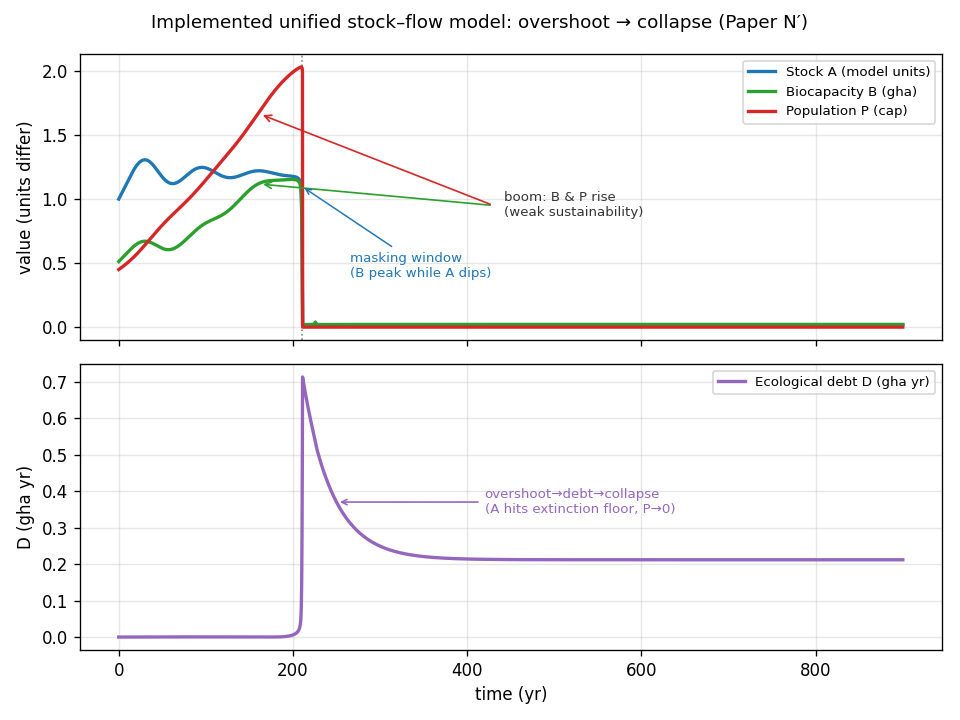
\includegraphics[width=0.8\textwidth]{S5_demo_overshoot_run.png}
\caption{One-stock comparator: top panel shows stock $A$ (model-specific stock units), population $P$ (cap) and annual biocapacity $B$ (gha); the lower panel shows leaky debt $D$ (gha\,yr). The footprint $E=eP$ is a driver and is not plotted. The shared numerical ordinate is illustrative, not a common physical scale. Comparator only; not a two-land result.}
\label{fig:si_s5}
\end{figure}

\begin{figure}[htbp]
\centering
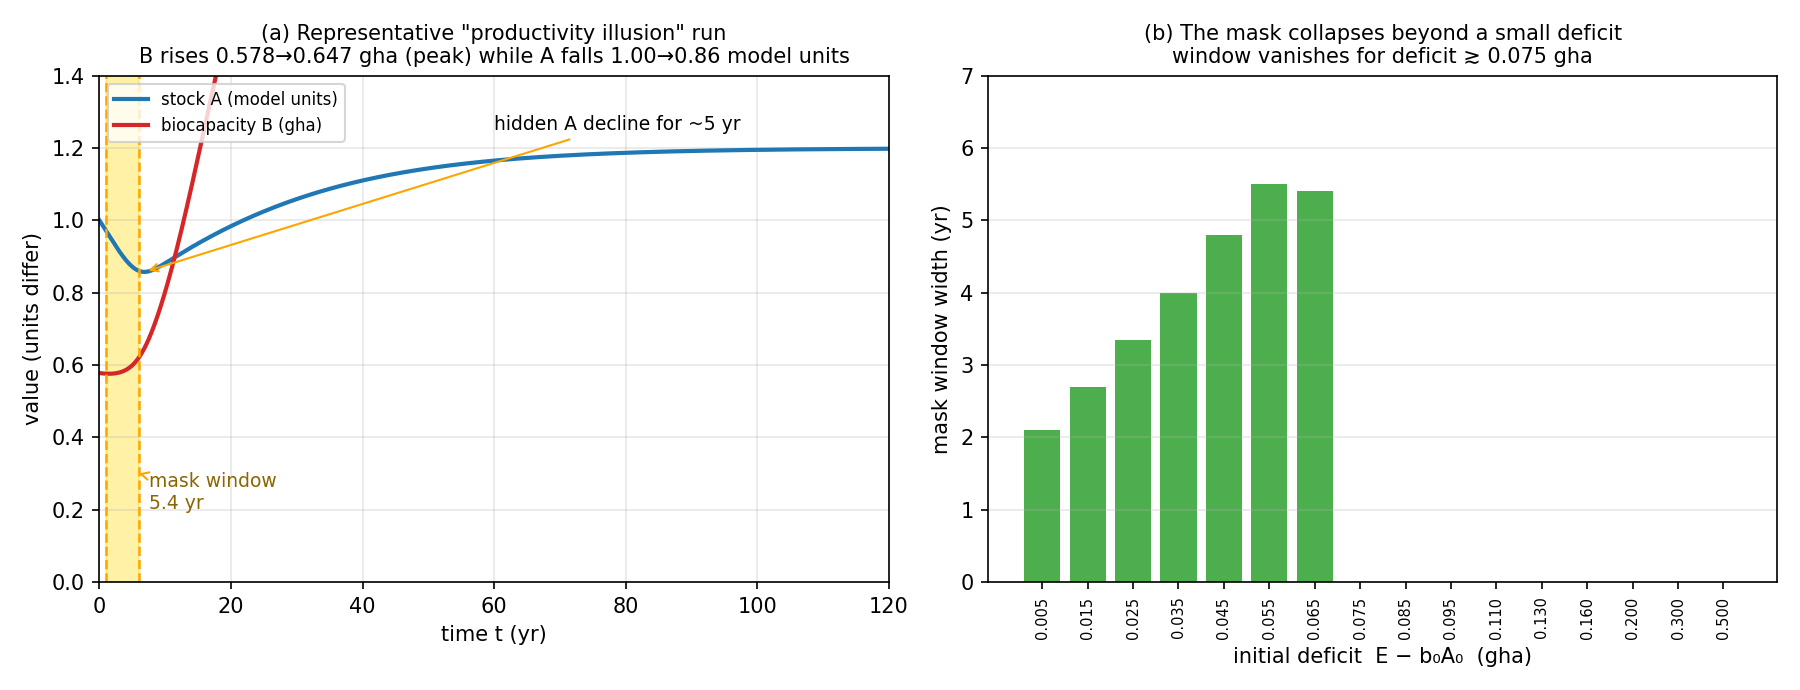
\includegraphics[width=0.8\textwidth]{S6_masking_window.png}
\caption{One-stock comparator: the productivity-illusion window ($A$ falls from $1.00$ to $0.86$ model units while $B$ rises from $0.578$ to $0.647$ gha; window $\approx5.4$\,yr; the mask vanishes for deficits $\gtrsim0.075$ gha). The two-land composition window of the paper (Fig.~1a) is a different object with a different mechanism.}
\label{fig:si_s6}
\end{figure}

\begin{figure}[htbp]
\centering
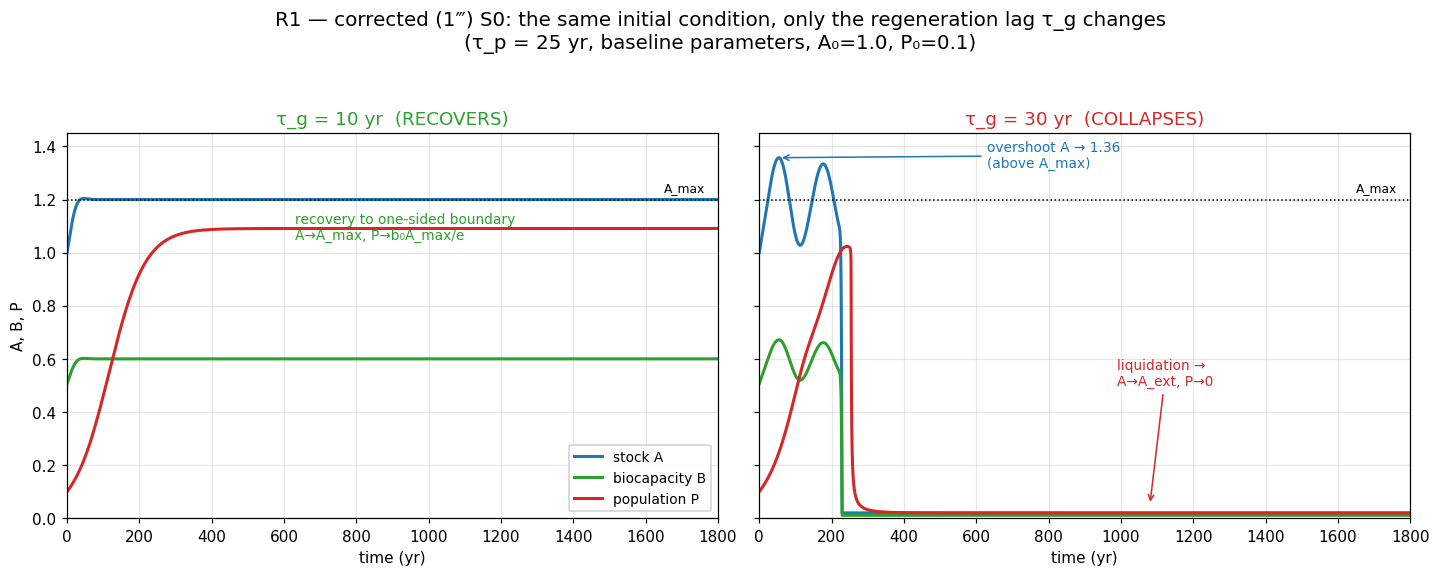
\includegraphics[width=0.8\textwidth]{S7_recovery_vs_collapse.png}
\caption{One-stock comparator: recovery versus collapse as a function of regeneration delay $\tau_g$ (yr; the $\approx18$--$20$\,yr cliff). The plotted series use a shared numerical ordinate only for illustration: stock $A$ is in comparator-specific units, biocapacity $B$ in gha and population $P$ in cap. Not present in the two-land model.}
\label{fig:si_s7}
\end{figure}

\begin{figure}[htbp]
\centering
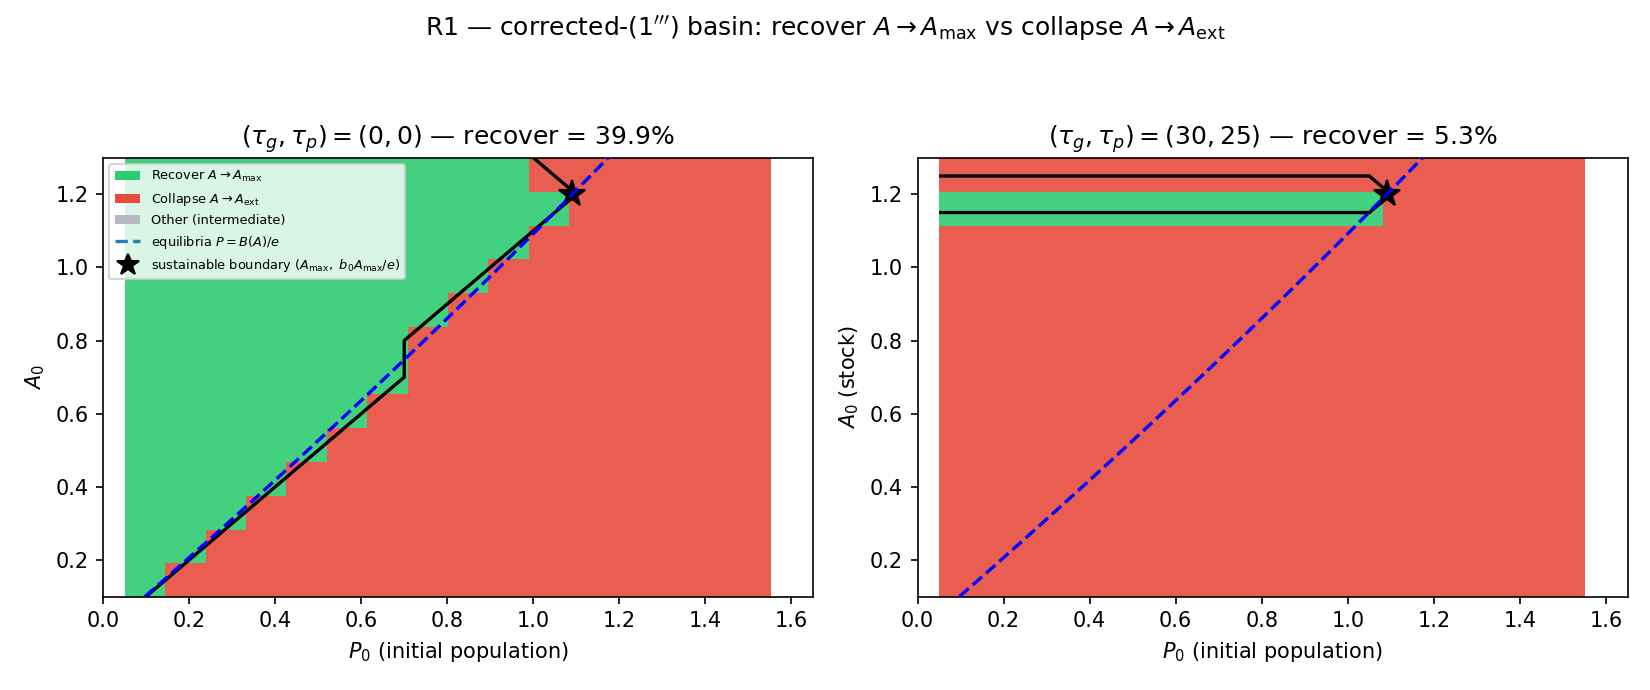
\includegraphics[width=0.8\textwidth]{S12_basin_baseline.png}
\caption{One-stock comparator: basin of recovery at the comparator baseline. The axes are initial population $P_0$ (cap) and initial stock $A_0$ (comparator-specific stock units); the equilibrium guide $P=B(A)/e$ is in cap, with annual account value $B$ in gha and $e$ in gha\,cap$^{-1}$. In the two-land model the corresponding object is the continuous drawdown-depth surface of Fig.~1c and Table~\ref{tab:si_drawdown}.}
\label{fig:si_s12}
\end{figure}

\section{Controlled technology-wave experiment}\label{si:tbwave}

This controlled extension tests whether an active $T_b$ wave can produce a larger leaky-debt peak than an otherwise matched no-wave run. The pair uses endogenous demand $E=eP$ (so the surplus-gated $R_{rc}$ is active only when $B>E$), $A_{tot}=2.5$\,ha, $A_{f0}=0.6$\,ha, $A_{c0}=0.9$\,ha, $q_0=0.9$, $D_0=0.0$\,gha\,yr, and $P_0=1.0$ or $1.2$\,cap. Shared parameters are $b_{f0}=0.85$\,gha\,ha$^{-1}$, $b_c=0.05$\,gha\,ha$^{-1}$, $b_{G,c}=0.8$\,gha\,yr\,ha$^{-1}$, $\rho_c=0.08$\,yr$^{-1}$, $\alpha=0.03$\,gha$^{-1}$\,yr$^{-1}$, $\eta=0.05$\,yr$^{-1}$, $\eta_f=0.05$\,yr$^{-1}$, $\mu=0.06$\,yr$^{-1}$, $e=0.55$\,gha\,cap$^{-1}$, $r=0.02$\,yr$^{-1}$, $\tau_g=20$\,yr, $\tau_p=25$\,yr, $\tau_{conv}=1$\,yr, and $\chi_r=0.10$\,gha$^{-1}$\,yr$^{-1}$. The wave parameters are $\Delta b=1.0$\,gha\,ha$^{-1}$, $\kappa_w=0.1$\,yr$^{-1}$, and $t_{wave}=40$\,yr; the horizon is $T=250$\,yr. Within each pair, the physical initial state, parameters, wave-free pre-run history, and solver are identical; only the $T_b$ switch differs. The logistic is already nonzero at $t=0$ ($T_b(0)=0.017986$\,gha\,ha$^{-1}$), so the derived initial account is $B(0)=0.560184$\,gha without the wave and $0.570976$\,gha with it. This small initial difference is part of the declared forcing, not a change to $A_f,A_c,q,P$, or $D$; $T_b$ reaches half its increment at the marked midpoint $t_{wave}=40$\,yr.

Figure~\ref{fig:si_wave_debt} shows the $P_0=1.0$ pair. Its all-time debt maximum occurs after the wave midpoint in both runs: $D_{max}=0.008126$\,gha\,yr at $86.15$\,yr without the wave, versus $0.020205$\,gha\,yr at $115.60$\,yr with it. At $P_0=1.2$, by contrast, the all-time maximum occurs early and is lower with the wave, while the maximum over $t\ge t_{wave}$ is higher. Table~\ref{tab:si_wave_debt} keeps these all-time and post-midpoint definitions separate. We call $t\ge t_{wave}$ the post-midpoint window; it is not an assertion that a logistic wave has ended at $t_{wave}$. The full metrics and trajectories are deposited as \texttt{work/tb\_wave\_debt\_metrics.csv}, \texttt{work/tb\_wave\_debt\_timeseries\_P0\_1p0.csv}, and \texttt{work/tb\_wave\_debt\_timeseries\_P0\_1p2.csv}; \texttt{work/tb\_wave\_debt\_scan.py} regenerates them and the figure.

\begin{table}[htbp]
\centering\small
\caption{Matched technology-wave/no-wave debt maxima. Entries are $D_{max}$ in gha\,yr, with the time of the maximum in years in parentheses; the ratio is wave/no-wave. ``All'' is the maximum over $0\le t\le250$\,yr; $t\ge40$ is the post-midpoint maximum. The $P_0=1.0$ all-time peaks both occur after the midpoint.}
\label{tab:si_wave_debt}
\begin{tabularx}{\textwidth}{r l r l >{\centering\arraybackslash}X >{\centering\arraybackslash}X r}
\toprule
$P_0$ (cap) & quality update & $\Delta t$ (yr) & window & no wave $D_{max}$ (time) & wave $D_{max}$ (time) & ratio \\
\midrule
$1.0$ & delayed & $0.050$ & all & $0.008126\ (86.15)$ & $0.020205\ (115.60)$ & $2.487$ \\
$1.0$ & delayed & $0.025$ & all & $0.008105\ (86.20)$ & $0.020195\ (115.65)$ & $2.492$ \\
$1.0$ & current & $0.050$ & all & $0.008326\ (85.70)$ & $0.020168\ (115.60)$ & $2.422$ \\
$1.2$ & delayed & $0.050$ & all & $0.061218\ (1.65)$ & $0.051037\ (1.45)$ & $0.834$ \\
$1.2$ & delayed & $0.050$ & $t\ge40$ & $0.010854\ (81.70)$ & $0.025184\ (112.55)$ & $2.320$ \\
$1.2$ & delayed & $0.025$ & all & $0.060732\ (1.625)$ & $0.050582\ (1.475)$ & $0.833$ \\
$1.2$ & delayed & $0.025$ & $t\ge40$ & $0.010808\ (81.775)$ & $0.025165\ (112.625)$ & $2.328$ \\
\bottomrule
\end{tabularx}
\end{table}

The $P_0=1.0$ result is a declared sensitivity case, not a refit or a universal effect: wave/no-wave all-time peak ratios persist under step halving ($2.487$ at $\Delta t=0.05$\,yr; $2.492$ at $0.025$\,yr) and under the current-quality solver ($2.422$ at $0.05$\,yr). At the reference $P_0=1.2$, the corresponding all-time ratios are $0.834$ and $0.833$, whereas the post-midpoint ratios are $2.320$ and $2.328$. All reported debt maxima change by less than $0.9\%$ under step halving. Maximum area-conservation residual is $4.44\times10^{-16}$\,ha; the minimum reserve in the $P_0=1.0$ wave run is $0.286$\,ha, above the $0.10$\,ha floor. In this sensitivity pair $A_c$ does not fall below its initial $0.9$\,ha, so the experiment isolates a debt rebound and is not evidence of the capital drawdown shown in the main frozen-demand run. The regression test also confirms that an integer input $D_0=0$ still produces a floating-point debt state and finite debt accumulation. $D$ is the model's leaky time-integral of shortfall, not an observed NFA or physical-stock variable. These conditional trajectories demonstrate a possible delayed rebound, while the $P_0=1.2$ contrast shows why the all-time peak cannot be substituted for the post-midpoint response.

\begin{figure}[!htbp]
\centering
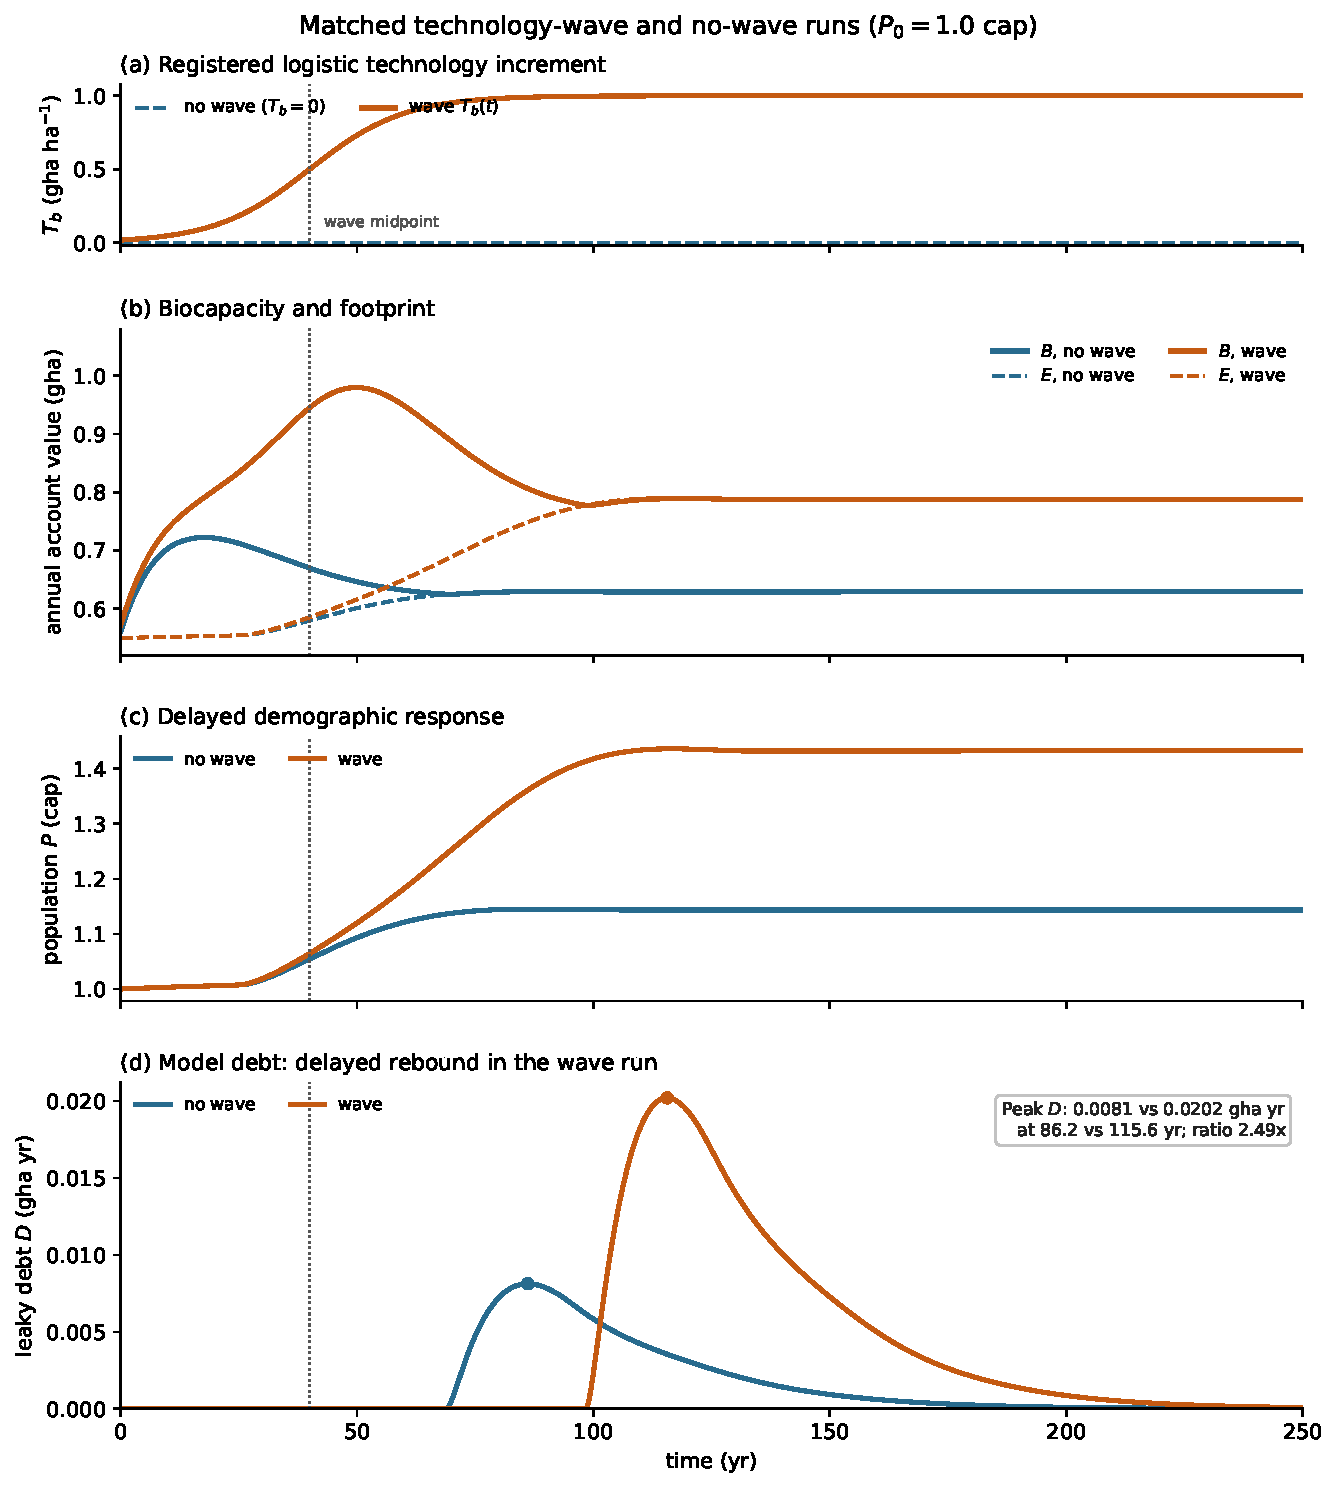
\includegraphics[width=0.92\textwidth]{fig_tb_wave_debt}
\caption{Matched endogenous-demand technology-wave/no-wave simulation at $P_0=1.0$\,cap. Parameters and initial conditions are listed in SI~\S S8; only $T_b$ is switched on or off. (a) The active logistic increment $T_b(t)$, with the dotted line at its midpoint $t_{wave}=40$\,yr; (b) annual account values $B$ and $E$ (gha); (c) population $P$ (cap); (d) leaky model debt $D$ (gha\,yr). Markers denote all-time maxima, which occur at $86.15$\,yr without the wave and $115.60$\,yr with it; peak debt is $0.008126$ versus $0.020205$\,gha\,yr. The plotted wave begins with its small logistic tail at $t=0$ and approaches $\Delta b=1.0$\,gha\,ha$^{-1}$; the dotted line marks the midpoint, not an end date.}
\label{fig:si_wave_debt}
\end{figure}

\section*{Supplementary references}
\begin{thebibliography}{99}
\small
\bibitem[{Abaee(2026a)}]{Abaee2026a} Abaee, A. (2026a). \emph{Governance delay and the stability of harvested stocks: mobilising and protective feedback rules, and the review interval as a design parameter.} Zenodo. \url{https://doi.org/10.5281/zenodo.22554217}.
\bibitem[{Abaee(2026b)}]{Abaee2026b} Abaee, A. (2026b). \emph{Aggregate Indices and Transition Safety: A Quantifier-Order Separation Between Scalarized and Coordinate-Wise Feasibility.} Zenodo. \url{https://doi.org/10.5281/zenodo.22545740}.
\bibitem[{Abaee(2026c)}]{Abaee2026c} Abaee, A. (2026c). \emph{Typed Flux Ledgers and Depletion Arithmetic: Conservation, Componentwise Diagnostics, and the Semantics of Depletion Horizons.} Zenodo. \url{https://doi.org/10.5281/zenodo.22554177}.
\bibitem[{Anderies(2000)}]{Anderies2000} Anderies, J. M. (2000). On modeling human behavior and institutions in simple ecological economic systems. \emph{Ecological Economics}, 35(3), 393--412.
\bibitem[{Becker et al.(2017)}]{Becker2017} Becker, W., Saisana, M., Paruolo, P. \& Vandecasteele, I. (2017). Weights and importance in composite indicators: Closing the gap. \emph{Ecological Indicators}, 80, 12--22.
\bibitem[{Blomqvist et al.(2013)}]{Blomqvist2013} Blomqvist, L., Brook, B. W., Ellis, E. C., Kareiva, P. M., Nordhaus, T. \& Shellenberger, M. (2013). Does the shoe fit? Real versus imagined ecological footprints. \emph{PLoS Biology}, 11(11), e1001700.
\bibitem[{Borucke et al.(2013)}]{Borucke2013} Borucke, M., Moore, D., Cranston, G., Gracey, K., Iha, K., Larson, J., Lazarus, E., Morales, J. C., Wackernagel, M. \& Galli, A. (2013). Accounting for demand and supply of the biosphere's regenerative capacity: The National Footprint Accounts' underlying methodology and framework. \emph{Ecological Indicators}, 24, 518--533.
\bibitem[{Brander and Taylor(1998)}]{BranderTaylor1998} Brander, J. A. \& Taylor, M. S. (1998). The simple economics of Easter Island: A Ricardo--Malthus model of renewable resource use. \emph{American Economic Review}, 88(1), 119--138.
\bibitem[{Calvin and Bond-Lamberty(2018)}]{CalvinBondLamberty2018} Calvin, K. \& Bond-Lamberty, B. (2018). Integrated human--Earth system modeling --- state of the science and future directions. \emph{Environmental Research Letters}, 13(6), 063006.
\bibitem[{Carvalhais et al.(2014)}]{Carvalhais2014} Carvalhais, N., Forkel, M., Khomik, M., Bellarby, J., Jung, M., Migliavacca, M., Mu, M., Saatchi, S., Santoro, M., Thurner, M., Weber, U., Ahrens, B., Beer, C., Cescatti, A., Randerson, J. T. \& Reichstein, M. (2014). Global covariation of carbon turnover times with climate in terrestrial ecosystems. \emph{Nature}, 514(7521), 213--217.
\bibitem[{Cohen(1995)}]{Cohen1995} Cohen, J. E. (1995). Population growth and Earth's human carrying capacity. \emph{Science}, 269(5222), 341--346.
\bibitem[{Copernicus(2019)}]{Copernicus2019} Copernicus (2019). \emph{Global Land Cover LC100.} European Commission, Land Copernicus.
\bibitem[{Dasgupta(2021)}]{Dasgupta2021} Dasgupta, P. (2021). \emph{The Economics of Biodiversity: The Dasgupta Review.} London: HM Treasury.
\bibitem[{Diamond(2005)}]{Diamond2005} Diamond, J. (2005). \emph{Collapse: How Societies Choose to Fail or Succeed.} New York: Viking.
\bibitem[{Donges et al.(2017)}]{Donges2017} Donges, J. F., Winkelmann, R., Cornell, S. E., Lucht, W., Dyke, J. G., Rockstr\"om, J., Heitzig, J. \& Schellnhuber, H. J. (2017). Closing the loop: Reconnecting human dynamics to Earth system science. \emph{The Anthropocene Review}, 4(2), 151--157.
\bibitem[{Erb et al.(2017)}]{Erb2017} Erb, K.-H., Luyssaert, S., Meyfroidt, P., Pongratz, J., Don, A., Kloster, S., Kuemmerle, T., Fetzel, T., Fuchs, R., Hasegawa, T., Haberl, H., et al. (2017). Land management: data availability and process understanding for global change studies. \emph{Global Change Biology}, 23(2), 512--533.
\bibitem[{ESA(2017)}]{ESA2017} ESA (2017). \emph{Land Cover CCI Product User Guide, Version 2.0.} European Space Agency.
\bibitem[{FAO(2020)}]{FAO2020} FAO (2020). \emph{Global Forest Resources Assessment 2020: Main Report.} Rome: Food and Agriculture Organization.
\bibitem[{FAO(2023)}]{FAO2023} FAO (2023). \emph{FAOSTAT: Land Use; Crops and Livestock Products.} Rome: Food and Agriculture Organization.
\bibitem[{Fischer et al.(2022)}]{Fischer2022} Fischer, S. M., Joy, M. K., Abrahamse, W., Milfont, T. L. \& Petherick, L. M. (2022). The use and misuse of composite environmental indices. \emph{bioRxiv}, 2022.03.15.484501. \url{https://doi.org/10.1101/2022.03.15.484501}.
\bibitem[{Global Footprint Network(2009)}]{GFNStandards2009} Global Footprint Network (2009). \emph{Ecological Footprint Standards 2009}. Global Footprint Network. \url{https://www.footprintnetwork.org/content/uploads/2019/05/Ecological_Footprint_Standards_2009.pdf}.
\bibitem[{Global Footprint Network(2019)}]{GFNGuidebook2019} Global Footprint Network (2019). \emph{Working Guidebook to the National Footprint Accounts 2019}. Global Footprint Network. \url{https://www.footprintnetwork.org/content/uploads/2019/05/National_Footprint_Accounts_Guidebook_2019.pdf}.
\bibitem[{Galli et al.(2016)}]{Galli2016} Galli, A., Giampietro, M., Goldfinger, S., Lazarus, E., Lin, D., Saltelli, A., Wackernagel, M. \& M\"uller, F. (2016). Questioning the ecological footprint. \emph{Ecological Indicators}, 69, 224--232.
\bibitem[{Giampietro and Saltelli(2014)}]{GiampietroSaltelli2014} Giampietro, M. \& Saltelli, A. (2014). Footprints to nowhere. \emph{Ecological Indicators}, 46, 610--621.
\bibitem[{Haberl et al.(2007)}]{Haberl2007} Haberl, H., Erb, K.-H., Krausmann, F., Gaube, V., Bondeau, A., Plutzar, C., Gingrich, S., Lucht, W. \& Fischer-Kowalski, M. (2007). Quantifying and mapping the human appropriation of net primary production in earth's terrestrial ecosystems. \emph{PNAS}, 104(31), 12942--12947.
\bibitem[{Henderson and Loreau(2018)}]{HendersonLoreau2018} Henderson, K. \& Loreau, M. (2018). How ecological feedbacks between human population and land cover influence sustainability. \emph{PLoS Computational Biology}, 14(8), e1006389.
\bibitem[{Hurtt et al.(2011)}]{Hurtt2011} Hurtt, G. C., Chini, L. P., Frolking, S., Betts, R. A., Feddema, J., Fischer, G., et al. (2011). Harmonization of land-use scenarios for the period 1500--2100: 600 years of global gridded annual land-use transitions, wood harvest, and resulting secondary lands. \emph{Climatic Change}, 109(1--2), 117--161.
\bibitem[{Hutchings and Reynolds(2004)}]{HutchingsReynolds2004} Hutchings, J. A. \& Reynolds, J. D. (2004). Marine fish population collapses: consequences for recovery and extinction risk. \emph{BioScience}, 54(4), 297--309.
\bibitem[{Hutchinson(1948)}]{Hutchinson1948} Hutchinson, G. E. (1948). Circular causal systems in ecology. \emph{Annals of the New York Academy of Sciences}, 50(4), 221--246.
\bibitem[{Klein Goldewijk et al.(2017)}]{KleinGoldewijk2017} Klein Goldewijk, K., Beusen, A., Doelman, J. \& Stehfest, E. (2017). Anthropogenic land use estimates for the last 12,000 years --- HYDE 3.2. \emph{Earth System Science Data}, 9(2), 927--953.
\bibitem[{Krausmann et al.(2013)}]{Krausmann2013} Krausmann, F., Erb, K.-H., Gingrich, S., Haberl, H., Bondeau, A., Gaube, V., Lauk, C., Plutzar, C. \& Searchinger, T. D. (2013). Global human appropriation of net primary production doubled in the 20th century. \emph{PNAS}, 110(25), 10324--10329.
\bibitem[{Kuang(1993)}]{Kuang1993} Kuang, Y. (1993). \emph{Delay Differential Equations, with Applications in Population Dynamics.} Academic Press.
\bibitem[{Lin et al.(2018)}]{Lin2018} Lin, D., Hanscom, L., Murthy, A., Galli, A., Evans, M., Neill, E., et al. (2018). Ecological footprint accounting for countries: updates and results of the National Footprint Accounts. \emph{Sustainability}, 10(12).
\bibitem[{May(1973)}]{May1973} May, R. M. (1973). \emph{Stability and Complexity in Model Ecosystems.} Princeton: Princeton University Press.
\bibitem[{Meadows et al.(1972)}]{Meadows1972} Meadows, D. H., Meadows, D. L., Randers, J. \& Behrens, W. W. (1972). \emph{The Limits to Growth.} New York: Universe Books.
\bibitem[{Meadows et al.(2004)}]{Meadows2004} Meadows, D. H., Randers, J. \& Meadows, D. L. (2004). \emph{The Limits to Growth: The 30-Year Update.} White River Junction, VT: Chelsea Green.
\bibitem[{Meadows et al.(1974)}]{Meadows1974} Meadows, D. L., Behrens, W. W., Meadows, D. H., Naill, R. F., Randers, J. \& Zahn, E. (1974). \emph{Dynamics of Growth in a Finite World.} Cambridge, MA: Wright-Allen Press.
\bibitem[{Meyer(1994)}]{Meyer1994} Meyer, P. S. (1994). Bi-logistic growth. \emph{Technological Forecasting and Social Change}, 47(1), 89--102.
\bibitem[{Meyer and Ausubel(1999)}]{MeyerAusubel1999} Meyer, P. S. \& Ausubel, J. H. (1999). Carrying capacity: A model with logistically varying limits. \emph{Technological Forecasting and Social Change}, 61(3), 209--214.
\bibitem[{Monfreda et al.(2008)}]{Monfreda2008} Monfreda, C., Ramankutty, N. \& Foley, J. A. (2008). Farming the planet: 2. Geographic distribution of crop areas, yields, physiological types, and net primary production in the year 2000. \emph{Global Biogeochemical Cycles}, 22(1), GB1022.
\bibitem[{Motesharrei et al.(2016)}]{Motesharrei2016} Motesharrei, S., Rivas, J., Kalnay, E., Asrar, G. R., Busalacchi, A. J., Cahalan, R. F., Cane, M. A., Colwell, R. R., Feng, K., Franklin, R. S., et al. (2016). Modeling sustainability: Population, inequality, consumption, and bidirectional coupling of the Earth and human systems. \emph{National Science Review}, 3(4), 470--494.
\bibitem[{Nardo et al.(2008)}]{Nardo2008} Nardo, M., Saisana, M., Saltelli, A., Tarantola, S., Hoffmann, A. \& Giovannini, E. (2008). \emph{Handbook on Constructing Composite Indicators: Methodology and User Guide.} Paris: OECD Publishing.
\bibitem[{Neubauer et al.(2013)}]{Neubauer2013} Neubauer, P., Jensen, O. P., Hutchings, J. A. \& Baum, J. K. (2013). Resilience and recovery of overexploited marine populations. \emph{Science}, 340(6130), 347--349.
\bibitem[{Pearl(1925)}]{Pearl1925} Pearl, R. (1925). \emph{The Biology of Population Growth.} New York: Alfred A. Knopf.
\bibitem[{Poeplau et al.(2011)}]{Poeplau2011} Poeplau, C., et al. (2011). Temporal dynamics of soil organic carbon after land-use change. \emph{Global Change Biology}, 17(7), 2415--2427.
\bibitem[{Poorter et al.(2016)}]{Poorter2016} Poorter, L., et al. (2016). Biomass resilience of Neotropical secondary forests. \emph{Nature}, 530(7590), 211--214.
\bibitem[{Schaefer(1954)}]{Schaefer1954} Schaefer, M. B. (1954). Some aspects of the dynamics of populations important to the management of the commercial marine fisheries. \emph{Bulletin of the Inter-American Tropical Tuna Commission}, 1(2), 25--56.
\bibitem[{Scheffer et al.(2001)}]{Scheffer2001} Scheffer, M., Carpenter, S., Foley, J. A., Folke, C. \& Walker, B. (2001). Catastrophic shifts in ecosystems. \emph{Nature}, 413(6856), 591--596.
\bibitem[{Simon(1996)}]{Simon1996} Simon, J. L. (1996). \emph{The Ultimate Resource 2.} Princeton: Princeton University Press.
\bibitem[{Tainter(1988)}]{Tainter1988} Tainter, J. A. (1988). \emph{The Collapse of Complex Societies.} Cambridge: Cambridge University Press.
\bibitem[{United Nations et al.(2021)}]{UN2021SEEA_EA} United Nations et al. (2021). \emph{System of Environmental-Economic Accounting---Ecosystem Accounting (SEEA EA).} White cover publication, pre-edited text subject to official editing. New York: United Nations. \url{https://seea.un.org/ecosystem-accounting}.
\bibitem[{United Nations(2022)}]{UN2022} United Nations (2022). \emph{World Population Prospects 2022: Summary of Results.} New York: Department of Economic and Social Affairs, Population Division.
\bibitem[{van den Bergh and Grazi(2015)}]{vdBerghGrazi2015} van den Bergh, J. C. J. M. \& Grazi, F. (2015). Reply to the first systematic response by the Global Footprint Network to criticism: a real debate finally? \emph{Ecological Indicators}, 58, 458--463.
\bibitem[{van den Bergh and Rietveld(2004)}]{vdBerghRietveld2004} van den Bergh, J. C. J. M. \& Rietveld, P. (2004). Reconsidering the limits to world population: Meta-analysis and meta-prediction. \emph{BioScience}, 54(3), 195--204.
\bibitem[{Wackernagel and Rees(1996)}]{WackernagelRees1996} Wackernagel, M. \& Rees, W. (1996). \emph{Our Ecological Footprint: Reducing Human Impact on the Earth.} New Society Publishers.
\bibitem[{Wackernagel et al.(2002)}]{Wackernagel2002} Wackernagel, M., et al. (2002). Tracking the ecological overshoot of the human economy. \emph{PNAS}, 99(14), 9266--9271.
\bibitem[{Wilson(2016)}]{Wilson2016} Wilson, E. O. (2016). \emph{Half-Earth: Our Planet's Fight for Life.} New York: Liveright.
\end{thebibliography}

\end{document}
